\documentclass[a4paper, 11pt, oneside]{extbook}\usepackage[T1]{fontenc}
\usepackage[utf8x]{inputenc}
\usepackage[italian]{babel} %Lingua italiana per gli standard e gli accenti
\usepackage{geometry}
\usepackage{courier}
\usepackage{pdfpages}
\newtheorem{example}{Esempio}[section]
\newtheorem{theorem}{Teorema}[section]
\newtheorem{prop}[theorem]{Proposizione}
\usepackage{amssymb}
%\usepackage{amsthm}
\usepackage{amsmath}
\usepackage{minted}
\usepackage{tikz}
\usepackage[bookmarks]{hyperref}
\newgeometry{
	left=   1.5 in,
	bottom= 1.5 in,
	right=  1 in,
	top=    1 in
}

\usepackage{fancyhdr}

% Grafica
\usepackage{graphicx,pstricks}
\usepackage{graphics}
\usepackage{subfigure}

%
%Algorithm
\usepackage{algorithm}
\usepackage[noend]{algpseudocode}

\setlength\headheight{44.2pt}
%Page Style
\usepackage{setspace}
%\setstretch{2.5} 
\doublespace
%
%%\cfoot{\thepage}
%\lhead[]{}
%\rhead[]{\leftmark}

\pagestyle{fancy}{
%	\lhead{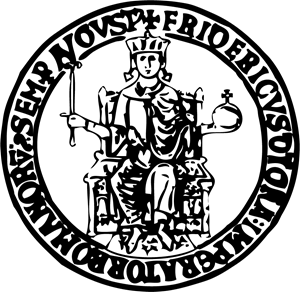
\includegraphics[scale=0.3]{img/logo.png}}
	%	\rhead{\footnotesize{\leftmark}}
	\rhead{\footnotesize{\leftmark}}
	%	\rfoot{\thepage}
}

%\fancyfoot[CE,CO]{\leftmark}
%\fancyfoot[LE,RO]{\thepage}
\renewcommand{\footrulewidth}{1pt}
\linespread{1}

%Other
\usepackage{comment}
\usepackage{amsmath}

%Testo riempitivo
\usepackage{lipsum}




\begin{document}
	\begin{titlepage}
	\begin{center}
		\vspace*{1cm}
		
		\Huge
		\textbf{Università degli Studi di Napoli \\ "Federico II"}
		
		\vspace{0.5cm}
		\LARGE
		Scuola Politecnica e delle Scienze di Base\\
		Corso di Laurea Magistrale in Ingegneria Informatica
		
		\vspace{1.5cm}
		
		\textbf{Giuseppe Francesco Di Cecio - M63001211}
		\\
		\textbf{Nicola D'Ambra - M63001223}
		
		\vspace{2cm}
		
		Elaborato di \textit{Calcolo Numerico}
		\\
		\vspace{0.5cm}
		\LARGE
		\textbf{Metodi Numerici per la risoluzione di Equazioni Differenziali Ordinarie (ODE)}
		\vfill
		
		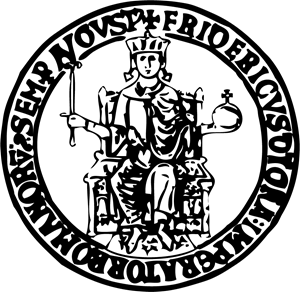
\includegraphics[width=0.2\textwidth]{img/logo.png}
		
		\Large
		Università degli Studi di Napoli \textit{Federico II}\\
		Napoli\\
		A.A 2020/2021
		
	\end{center}
\end{titlepage}
	\frontmatter						%Numerazione romana
	

	{\setstretch{1.5}					%Indice
		\tableofcontents
	}
	
	\backmatter							%Inizio numerazione capitoli
	\mainmatter							%Numerazione pagine
	\chapter[Metodo di Eulero]{Metodo di Eulero - Esplicito}

Il metodo di Eulero è un semplice algoritmo per ricavare una soluzione numerica ad'\textit{equazione differenziale ordinaria} (ODE).
Sia il seguente problema di Cauchy:
\begin{equation}
	\label{ode}
	\begin{cases}
		\dfrac{dy}{dt} = f(t,y(t)) \\[0.2cm]
		y(t_{0}) = y_{0}
	\end{cases}
\end{equation}
con $t \in I = [t_{0},T]$ e $T$ prefissato.
\\Prima di procedere con la descrizione della tecnica si può fare una breve ripresa del concetto di Serie di Taylor.

\section{Serie di Taylor}
La serie di Taylor di una funzione in un punto è la rappresentazione della funzione come serie di termini calcolati a partire dalle derivate della funzione stessa nel punto.
\\Sia $f(x)$ definita a valori reali, o complessi, infinite volte derivabile, la serie di Taylor centrata nel punto $x_0$ è la seguente serie di potenze:
\begin{equation*}
	f(x) = f(x_{0}) + f'(x_{0})(x-x_{0}) + \dfrac{f''(x_{0})}{2}(x-x_{0})^{2}	+ \dfrac{f'''(x_{0})}{6}(x-x_{0})^{3} + ...
\end{equation*} 
In generale:
\begin{equation}
	f(x) = \sum_{n=0}^{\infty} \dfrac{f^{(n)}(x_{0})}{n!}(x-x_{0})^{n}
\end{equation}
A questo punto si può continuare con la descrizione.
\vspace{0.5cm}
\\Si discretizza l'intervallo $I$ in $n$ sottointervalli:
\begin{figure}[H]
	\centering
	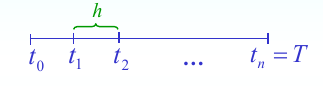
\includegraphics[width=0.4\textwidth]{img/discretizzazione.png}
\end{figure}
In modo che:
\begin{equation*}
	t_{i} = t_{i-1}+h \qquad h = \dfrac{T-t_{0}}{n}
\end{equation*}
La funzione soluzione $y(t)$ viene approssimata alla serie di Taylor arrestata al primo ordine, in ogni intervallo. In generale vale la seguente uguaglianza:
\begin{equation*}
	y(x) = y(x_{0}) + y'(x_{0})(x-x_{0}) + R(x, x-x_{0})
\end{equation*}
Trascurando il resto $R(x, x-x_{0})$, nel caso in esame:
\begin{equation*}
	h = x-x_{0} \qquad t_{i}=x_{0}
\end{equation*}
si ha:
\begin{equation*}
	y(t_{i}+h) \approx y(t_{i}) + y'(t_{i})h
\end{equation*}
Per la \ref{ode}:
\begin{equation}
	y(t_{i}+h) \approx y(t_{i}) + f(t_{i}, y(t_{i}))h
\end{equation}
Quindi la funzione soluzione può essere ricava in corrispondenza di ogni punto $t_i$ dell'intervallo $I$ come:
\begin{enumerate}
	\item $y(t_{0}) \approx y_{0}$
	\item $ y(t_1) = y(t_0+h) \approx y(t_{0}) + f(t_{0}, y(t_0)) h$
	\item $y(t_2) = y(t_1+h) \approx  y(t_{1}) + f(t_{1}, y(t_1)) h$
\item ...
\end{enumerate}
In generale quindi::
\vspace{0.5cm}
\\
\fbox{\parbox{\textwidth}{
		\vspace{0.5cm}
		\qquad Noto $y_0$, la \textbf{legge di aggiornamento} vale:
		\begin{equation}
			\label{eulero}
			y_{i+1} = y_i + f(t_i, y_i)h \quad \forall i \in \{0,1,2,...,n-1\}
		\end{equation}
		\qquad con $y_i \approx y(t_{i})$ una stima del reale valore della funzione soluzione.
		\\
	}
}
\section{Interpretazione Geometrica}
Dalla \ref{eulero} si può intuire che in un intervallo qualsiasi $[t_i, t_{i+h}]$, con $h$ passo di discretizzazione, la funzione soluzione $y(t)$ viene approssimata ad una retta tangente nel punto $t_i$, centro dello sviluppo di Taylor arrestato al primo ordine. 
\begin{figure}[H]
	\centering
	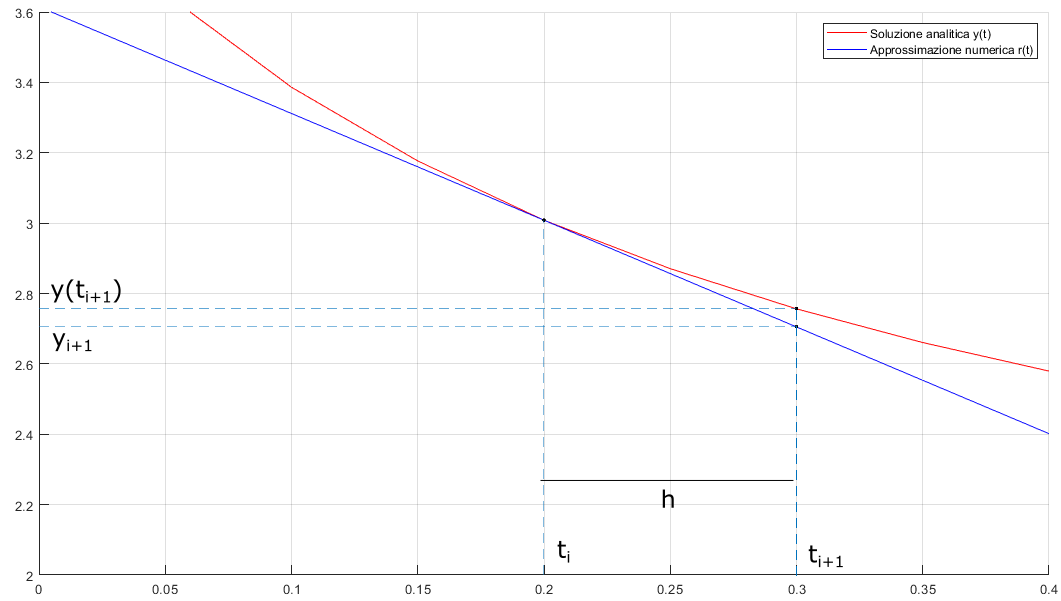
\includegraphics[width=\textwidth]{matlab/interpretazione_geometrica.png}
	\caption{\textit{Confronto tra soluzione numerica e soluzione analitica}}
\end{figure}
Sia la retta $r(t)$:
\begin{equation*}
	r(t) = y(t_i)+f(t_i,y(t_i))(t-t_i)
\end{equation*}
e $y(t)$ soluzione analitica, al passo $(i+1)-esimo$ si approssima:
\begin{equation*}
	y(t_{i+1}) \approx y_{i+1} = r(t_{i+1})
\end{equation*}

\section{Implementazione Matlab}
L'implementazione in Matlab è molto semplice. Prevede infatti solo la realizzazione della legge di aggiornamento della soluzione numerica.
\\I parametri di ingresso alla funzione sono:
\begin{itemize}
	\item \textbf{$f$} Funzione dell'equazione differenziale di tipo \ref{ode}
	\item \textbf{$y_0$} Condizione iniziale al tempo $t_0$
	\item \textbf{$t_0$} Tempo iniziale
	\item \textbf{$T$} Tempo finale
	\item \textbf{$h$} Passo di discretizzazione
\end{itemize}
I parametri in uscita sono:
\begin{itemize}
	\item \textbf{$t$} Asse dei tempi discretizzato
	\item \textbf{$y$} Vettore soluzione
\end{itemize}
Il metodo di Eulero può essere implementato sia in un sistema aritmetico a \textit{singola precisione} che in \textit{doppia precisione}.
\begin{itemize}
	\item \textbf{eulero32} implementazione del metodo con calcoli in \textit{singola precisione} a 32bit.
	\item \textbf{eulero64} implementazinoe del modello con calcoli in \textit{doppia precisione} a 64bit
\end{itemize}
\begin{minted}[framesep = 1mm,
	fontsize = \footnotesize,
	]{MATLAB}
function [y, t] = eulero32(f, y0, t0, T, h)
	t = single(t0:h:T);                 %Asse dei tempi discretizzata con passo h
	y = single(zeros(1,length(t)));     %Vettore soluzione
	y(1) = y0;                  %Condizione iniziale
	
	for i=1:length(t)-1
		y(i+1) = y(i) + f(t(i), y(i))*h;    %Costruzione della soluzione
	end
end
\end{minted}
\begin{minted}[framesep = 1mm,
	fontsize = \footnotesize,
	]{MATLAB}
function [y, t] = eulero64(f, y0, t0, T, h)
	t = t0:h:T;                 %Asse dei tempi discretizzata con passo h
	y = zeros(1,length(t));     %Vettore soluzione
	y(1) = y0;                  %Condizione iniziale
	
	for i=1:length(t)-1
		y(i+1) = y(i) + f(t(i), y(i))*h;    %Costruzione della soluzione
	end
end
\end{minted}
\begin{example}
	Sia la seguente equazione differenziale	con $t \in [0,1]$:
	\begin{equation*}
		\begin{cases}
			\dfrac{dy}{dt} = 2y(t)-y^2(t) \\[0.2cm]
			y(t_{0}) = 4
		\end{cases}
	\end{equation*}
	La soluzione analitica è la seguente:
	\begin{equation*}
		y(t) = \dfrac{4}{2-e^{-2t}}
	\end{equation*}
	La soluzione numerica può essere calcolata con la funzione MATLAB descritta precedentemente:
	\begin{minted}[framesep = 1mm,
		fontsize = \footnotesize,
		]{MATLAB}
f = @(t,y) 2*y-y^2;
t0 = 0;
T = 1;
[y_eulero,t] = eulero64(f, 4, t0, T, 0.05);
y_analitica = 4./(2-exp(-2.*t));
hold on;
grid;
plot(t,y_eulero);
plot(t, y_analitica);
legend('Soluzione numerica (Eulero)', 'Soluzione analitica');
	\end{minted}
Il cui risultato è il seguente:
\begin{figure}[H]
	\centering
	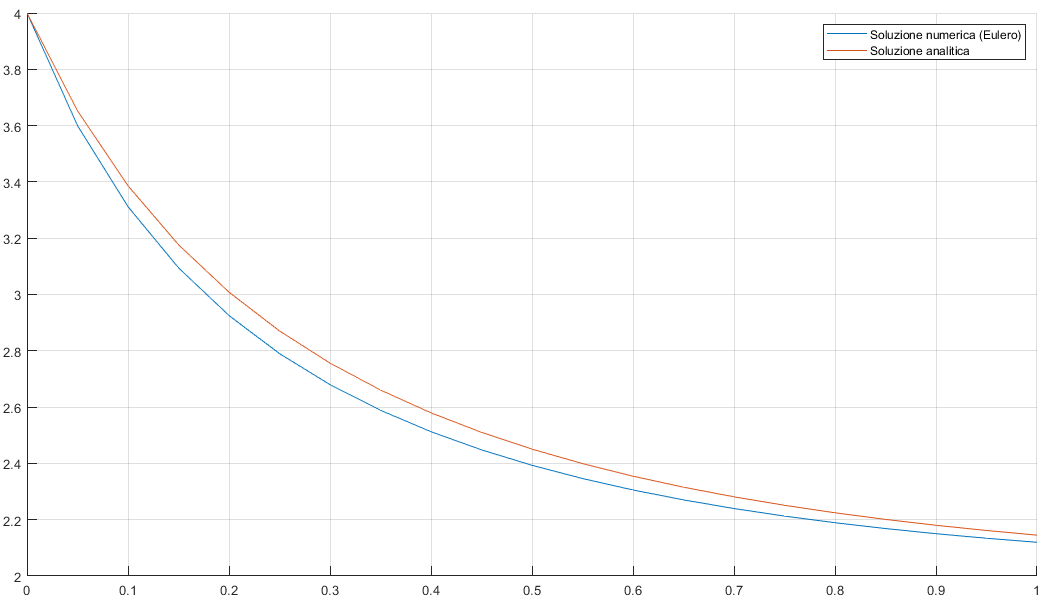
\includegraphics[width=\textwidth]{matlab/esempio1_eulero.png}
	\caption{\textit{Soluzione numerica con passo di discretizzazione h=0.05}}
\end{figure}
\end{example}

\section{Errori}
La legge di aggiornamento specifica che:
\begin{equation*}
	y_i \approx y(t_i)
\end{equation*}
quindi il metodo da luogo a degli errori.
\\Una soluzione numerica presenta sempre degli errori rispetto alla relativa soluzione analitica. Alcuni dovuti a delle approssimazioni altre invece a causa dell'elaborazione in un sistema aritmetico a precisione finita.



\subsection{Errore di Discretizzazione}
Sia il seguente problema di Cauchy del primo ordine:
\begin{equation*}
	M(P) :
	\begin{cases}
		\dfrac{dy}{dt} = f(t, y(t)) \\[0.2cm]
		y(t_{0}) = y_0
	\end{cases}
\end{equation*}
Data la legge di aggiornamento \ref{eulero} si ha:
\begin{equation*}
	y_{i+1} = y_i +f(t_i, y_i)h \quad \Rightarrow \quad \dfrac{y_{i+1}-y_i}{h} = f(t_i,y_i)
\end{equation*}
ovvero la derivata viene sostituita con il rapporto incrementale, avendo così un problema discretizzato con passo $h$:
\begin{equation}
	M_h(P) :
	\begin{cases}
		\dfrac{y_{i+1}-y_i}{h} = f(t_i,y_i) \qquad \forall i = \{0,1,...,n-1\} \\[0.2cm]
		y(t_{0}) = y_0
	\end{cases}
\end{equation}
commettendo un \textbf{errore di discretizzazione}.
\\In generale l'errore viene definito come la differenza tra l'approssimazione e il valore reale. Nel caso del metodo di Eulero, quindi, l'errore è la differenza tra il rapporto incrementale e la derivata nel punto $t$:
\begin{equation*}
	T(t,h) = \dfrac{y(t+h)-y(t)}{h} - y'(t)
\end{equation*}
ovvero:
\begin{equation}
	T(t,h) = \dfrac{y(t+h)-y(t)}{h} - f(t,y(t))
\end{equation}
Quindi l'errore di discretizzazione è la "distanza" tra il problema continuo $M(P)$ e il problema discreto $M_h(P)$.
\\Inoltre tale errore misura l'\textbf{accuratezza} fornita dal metodo.

\subsubsection{Consistenza}
Un metodo per la risoluzione di un problema ai valori iniziali si dice \textbf{consistente} se, fissato $t$:
\begin{equation*}
	\lim_{h \rightarrow 0} T(t,h) = 0
\end{equation*}
ovvero se l'errore di discretizzazione tende a 0, al tendere a 0 del passo di discretizzazione $h$.
\\La consistenza esprime il fatto che il problema discreto è una buona approssimazione del problema continuo:
\begin{equation*}
	\lim_{h \rightarrow 0} M_h(P) = M(P)
\end{equation*}
Inoltre un metodo di risoluzione si dice \textbf{consistente (o accurato) di ordine \textit{p}} se:
\begin{equation}
	T(t,h) = O(h^p)
\end{equation}
\hrule
\vspace{0.5cm}
Il problema discretizzato con il metodo di Eulero $M_h(P)$ è una buona approssimazione del problema continuo $M(P)$, poiché:
\begin{equation*}
	\lim_{h \rightarrow 0} T(t,h) = \lim_{h \rightarrow 0} \dfrac{y(t+h)-y(t)}{h} - y'(t) = 0
\end{equation*} 
Il rapporto incrementale tende alla derivata per $h \rightarrow 0$.
\\Il metodo di Eulero è consistente di ordine 1.

\subsection{Errore di Troncamento Locale}
L'errore di troncamento locale (LTE) equivale a:
\begin{equation}
	\label{lte}
	\tau_i = y(t_i) - y_i \quad con \quad y_j = y(t_j) \quad\forall j <i 
\end{equation}
calcolato assumendo che tutti i precedenti valori numerici ad $i$ siano accurati.
\\Il metodo di Eulero approssima la funzione soluzione alla sua serie di Taylor arrestata al primo ordine:
\begin{equation*}
	\begin{cases}
		y(t_{i+1}) = y(t_i+h) = y(t_i) + f(t_i, y(t_i))h + O(h^2) \\
		y_{i+1} = y_i + f(t_i, y_i)h
	\end{cases}
\end{equation*}
Assumendo la condizione che le soluzioni numeriche precedenti al passo $i$ siano coincidenti con quelle analitiche, la \ref{lte} per il metodo di Eulero vale:
\begin{equation}
	\tau_{i+1} = y(t_{i+1}) - y_{i+1} = O(h^2)
\end{equation}

\subsection{Errore di Troncamento Globale}
Il metodo di Eulero è un metodo consistente, in cui il problema $M_h(P)$ è una buona approssimazione del problema $M(P)$.
\\Analizzando le soluzioni dei due problemi:
\begin{equation*}
	\begin{split}
		M(P) & \quad \rightarrow \quad y(t) \\
		M_h(P) & \quad \rightarrow \quad (y_0, y_1, ..., y_{n-1}) 	
	\end{split}
\end{equation*}
bisogna capire se la soluzione discreta è una buona approssimazione della soluzione continua calcolata negli stessi punti:
\begin{equation*}
	\begin{split}
		y_0 &\approx y(t_0) \\
		y_1 & \approx y(t_1) \\
		... &\approx ... \\
		y_{n-1} &\approx y(t_{n-1})
	\end{split}
\end{equation*}
Data la funzione $u: [t_0, T] \rightarrow \mathbb{R}$ tale che:
\begin{equation}
	u(t_i) = y_i \qquad \forall i = {0,1,...,n-1}
\end{equation}
essa è soluzione del problema $M_h(P)$:
\begin{equation*}
	M_h(P) :
	\begin{cases}
		\dfrac{u(t_{i+1})-u(t_i)}{h} = f(t_i,u(t_i))  \\[0.2cm]
		u(t_{0}) = y(t_0)
	\end{cases}
\qquad \forall i = \{0,1,...,n-1\}
\end{equation*}
mentre $y(t)$ è soluzione del problema continuo:
\begin{equation*}
	M(P) :
	\begin{cases}
		y'(t) = f(t,y(t)) \\[0.2cm]
		y(t_{0}) = y_0
	\end{cases}
\quad \forall t \in [t_0,T]
\end{equation*}
L'\textbf{errore globale di troncamento} (GTE) viene definito come:
\begin{equation}
	E_i(h) = y(t_i) - u(t_i) \quad \forall i = \{0,1,...,n-1\}
\end{equation}
ovvero al passo $i-esimo$ l'errore è la differenza tra la soluzione discreta e quella analitica, e misura l'\textit{accuratezza} della soluzione numerica.
\\A differenza dell'errore di troncamento locale, in questo caso si tiene conto degli errori commessi negli step precedenti al passo $i-esimo$.
\\Una stima dell'errore di troncamento globale all'utimo step $N-esimo$ può essere calcolata nel seguente modo:
\begin{equation}
	\label{GTE}
	E_N \approx N \tau_i = N O(h^2) \approx O(h)
\end{equation}
Dato che è noto l'errore in ogni step.
\subsubsection{Convergenza}
Un metodo per la risoluzione di un problema ai valori iniziali si dice \textbf{convergente} se, posto $E_0=0$:
\begin{equation*}
	\begin{cases}
		E_0 = y(t_0) - u(t_0) \\
		u(t_0) = y(t_0)
	\end{cases}
\Rightarrow \quad E_0 = y(t_0)-y(t_0)=0
\end{equation*} 
fissato $t = t_0 + ih$ risulta:
\begin{equation*}
	\lim_{h \rightarrow 0} E_i(h) = 0 \qquad opp. \qquad \lim_{i \rightarrow \infty	} E_i(h) = 0 
\end{equation*}
Inoltre un metodo si dice \textbf{convergente di ordine \textit{p}} se risulta:
\begin{equation}
	E_i(h) = O(h^p)
\end{equation}
La convergenza esprime il fatto che la soluzione del problema discreto è una buona approssimazione della soluzione del problema continuo. La \ref{GTE} non è sufficiente nel dimostrare che il metodo è convergente.

\begin{theorem}
	Sia $y(t)\in C^2[t_0,T]$ soluzione del problema $M(P)$. Sia inoltre $y(t)$ Lipschitziana di costante $L$ in ogni intervallo $[t_i, t_{i+1}]$, ovvero:
	\begin{equation*}
		|y(t_i) - y(t_{i+1})| \leq L |t_i - t_{i+1}| \quad \Rightarrow \quad \dfrac{|y(t_i) - y(t_{i+1})|}{|t_i - t_{i+1}|} \leq L \quad \quad \forall i\in \{0,1,...,n-1\}
	\end{equation*}
	ovvero che la pendenza in ogni intervallo non superi una determinata angolazione.
	\\L'errore di troncamento globale viene calcolato come:
	\begin{equation*}
		|E_i(h)| \leq e^{(T-t_0)L}|E_0| + \dfrac{e^{(T-t_0)L}-1}{L}\dfrac{C}{2}h
	\end{equation*}
	con \[ C=
	\max_{[t_0,T]} 
	 y''(t) \]
\end{theorem}
Ponendo $E_0=0$ si ha:
\begin{equation}
	\label{gte}
	|E_i(h)| \leq \dfrac{Ce^{(T-t_0)L}-1}{2L}h \approx O(h)
\end{equation}
quindi il metodo di Eulero è \textbf{convergente di ordine 1}.

\begin{example}
Sia la seguente equazione differenziale	con $t \in [0,1]$:
\begin{equation*}
	\begin{cases}
		\dfrac{dy}{dt} = -2y(t)+1 \\[0.2cm]
		y(t_{0}) = 1
	\end{cases}
\end{equation*}
La soluzione analitica è la seguente:
\begin{equation*}
	y(t) = \dfrac{e^{-2t}+1}{2}
\end{equation*}
Uno script per valutare l'errore è il seguente:
\begin{minted}[framesep = 1mm,
	fontsize = \footnotesize,
	]{MATLAB}
	%Eq. Differenziale
	f = @(t,y) -2*y+1;
	%Dati iniziali
	t0 = 0;
	y0 = 1;
	T = 1;
	h = [0.2 0.1 0.05];
	global_error = zeros(3,1);
	
	%Soluzione analitica da confrontare
	t = 0:0.001:1;
	y_analitica = (exp(-2.*t)+1)./2;
	plot(t,y_analitica);
	
	hold on;
	grid;
	%Calcolo delle soluzioni numeriche
	for i=1:3
		[y_eulero,t] = eulero(f, y0, t0, T, h(i));
		y_analitica = (exp(-2.*t)+1)./2;
		plot(t,y_eulero);
		global_error(i,1) = max(y_analitica-y_eulero)
	end
	legend( 'Soluzione analitica','h=0.2', 'h=0.1', 'h=0.05');
\end{minted}
Il cui risultato è il seguente:
\begin{figure}[H]
	\centering
	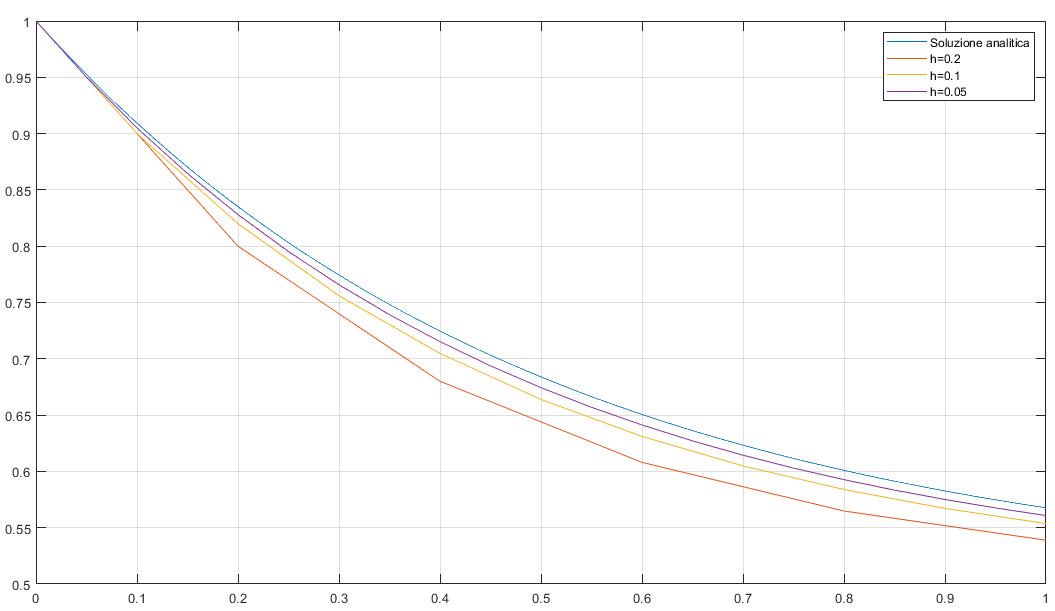
\includegraphics[width=\textwidth]{matlab/errore_troncamento_globale.png}
	\caption{\textit{Confronto delle soluzioni numeriche}}
\end{figure}
Il vettore global\_error =
	$\begin{pmatrix}
		0.44 \times 10^{-1} & 0.20 \times 10^{-1} & 0.96 \times 10^{-2}
	\end{pmatrix}$
\end{example}
Come si nota dall'esempio se si vuole dimezzare l'errore (raddoppiare la precisione) bisogna dimezzare anche il passo di discretizzazione $h$.
\\In termini computazionali il problema è notevole. Se si vuole avere una precisione tale che $h=10^{-8}$ allora:
\begin{equation*}
	N = \dfrac{T}{h} \approx 10^8 
\end{equation*}
Il che richiede dunque un gran numero di iterazioni per risolvere un problema.

\subsection{Errore di Rounf-Off}
La soluzione discreta viene calcolata all'interno di un sistema aritmetico a precisione finita (computer) quindi è soggetta ad un errore di round-off.
\\Indicando con $\tilde{u}(t_i)$ il valore della soluzione discreta $u(t_i)$ calcolata in un sistema aritmetico floating-point, l'\textbf{errore globale di round-off} viene definito come:
\begin{equation}
	R_i(h) = u(t_i) - \tilde{u}(t_i)
\end{equation}
\begin{theorem}
	Sia $u(t_i)$ Lipschitziana e soluzione del problema discreto $M_h(P)$ l'errore globale di round-off del metodo di Eulero, vale:
	\begin{equation}
		\label{roundoff}
		|R_i(h)| \leq e^{(T-t_0)L}|R_0| + \dfrac{e^{(T-t_0)L}-1}{L}\dfrac{\rho}{h} 
	\end{equation}
dove $R_0$ indica l'errore di round-off nel dato iniziale e:
\[
	\rho = \max_{i}(\rho_i)
\]
in cui $\rho_i$ è l'errore locale di round-off commesso al passo $i-esimo$.
\end{theorem}
Dal teorema si deduce che al crescere di $h$ diminuisce l'errore di round-off globale.
\\Tale affermazione va però contro la \ref{gte}, in cui l'errore globale diminuisce alla diminuzione di $h$.

\subsection{Errore Totale}
L'errore totale è l'errore che tiene in considerazione sia l'errore globale di round-off sia l'errore globale di troncamento. Per adesso quindi:
\begin{equation*}
	\begin{cases}
		|E_i(h)| \leq e^{(T-t_0)L}|E_0| + \dfrac{e^{(T-t_0)L}-1}{L}\dfrac{C}{2}h \\[0.4cm]
		|R_i(h)| \leq e^{(T-t_0)L}|R_0| + \dfrac{e^{(T-t_0)L}-1}{L}\dfrac{\rho}{h} 
	\end{cases}
\end{equation*}
In entrambi i casi il primo addendo riguarda l'accumulo dell'errore a partire da quello iniziale, mentre il secondo addendo riguarda l'accumulo degli errori locali. Se $h$ diminuisce:
\begin{itemize}
	\item L'errore globale di round-off $R_i(h)$ \underline{cresce}
	\item L'errore globale di troncamento $E_i(h)$ \underline{decresce}
\end{itemize}
L'errore totale è definito come:
\begin{equation}
	\label{total_error}
	E^{tot}_i(h) = |y(t_i) - \tilde{u}(t_i)|
\end{equation}
differenza della soluzione $i-esima$ del problema continuo $M(P)$ e soluzione discreta in un sistema a precisione finita. Sommando e sottraendo alla \ref{total_error} la quantità $u(t_i)$ si ha:
\begin{equation}
	\label{e_tot}
E^{tot}_i(h) = |y(t_i) - u(t_i) + u(t_i) - \tilde{u}(t_i)| = |E_i(h) + R_i(h)| \leq |E_i(h)| + |R_i(h)|
\end{equation}
combinando quindi tutte le equazioni:
\begin{equation}
	E^{tot}(h) \leq e^{(T-t_0)L}\left(|E_0|+|R_0|\right) + \dfrac{e^{(T-t_0)L}-1}{L}\left(\dfrac{C}{2}h + \dfrac{\rho}{h}\right)
\end{equation}
\begin{figure}[H]
	\centering
	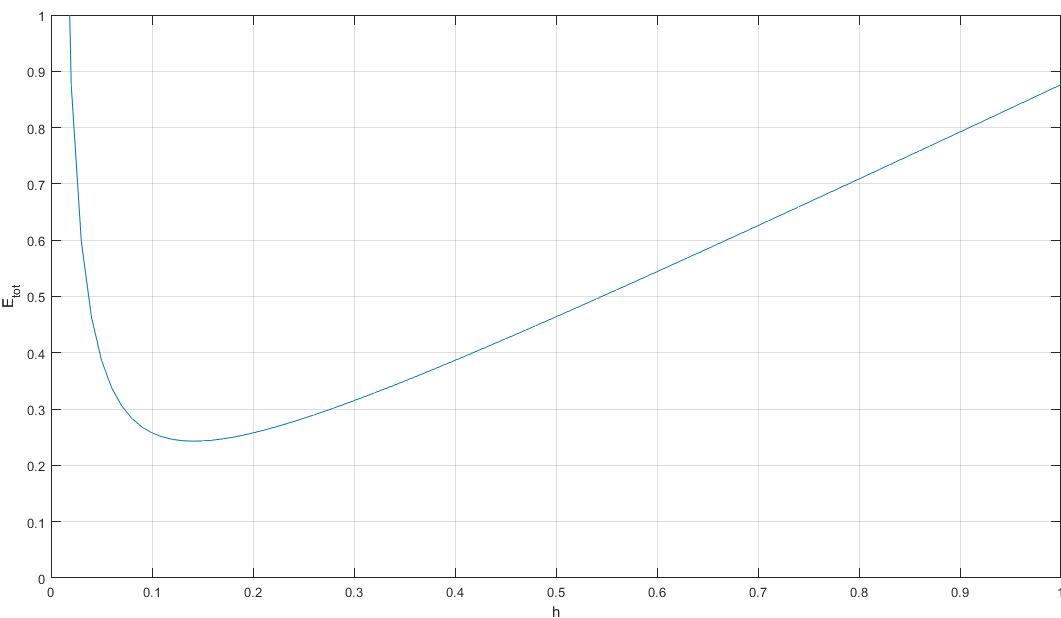
\includegraphics[width=\textwidth]{matlab/errore_totale.png}
	\caption{\textit{Errore totale in funzione di h}}
	\label{e_tot_fig}
\end{figure}
Il valore ottimo di $h$ è quello che minimizza la funzione $E^{tot}(h)$. Calcolando quindi il valore per cui:
\begin{equation*}
	\dfrac{dE^{tot}(h)}{dh} = 0 \quad \Rightarrow \quad \dfrac{C}{2L}h_{opt} = \dfrac{\rho}{L}\dfrac{1}{h_{opt}}
\end{equation*}
in definitiva:
\vspace{0.5cm}
\\
\fbox{\parbox{\textwidth}{
		\begin{equation*}
			h_{opt} = \sqrt{\dfrac{2\rho}{C}}
		\end{equation*}
	}
}
\vspace{0.5cm}
\\
Il valore sopra calcolato in realtà è un valore teorico. La funzione soluzione $y(t)$ infatti non è conosciuta il più delle volte, non potendo quindi calcolare $\rho$ e $C$.


\section{Stabilità}
L'algoritmo di Eulero è un metodo \textit{consistente} e \textit{convergente}. In generale, però, il valore $h$ scelto per ricavare la soluzione indice molto sulla stessa. Per valori di $h$ abbastanza grandi, infatti, l'errore potrebbe divergere rendendo la soluzione inaccettabile.

\begin{example}
	Sia la seguente equazione differenziale	con $t \in [0,0.8]$:
	\begin{equation*}
		\begin{cases}
			\dfrac{dy}{dt} = -15y(t) \\[0.2cm]
			y(t_{0}) = 0.6
		\end{cases}
	\end{equation*}
	La soluzione analitica è la seguente:
	\begin{equation*}
		y(t) = 0.6 e^{-15t}
	\end{equation*}
	Calcolando la soluzione numerica con vari valori di $h$ si ha:
	\begin{figure}[H]
		\centering
		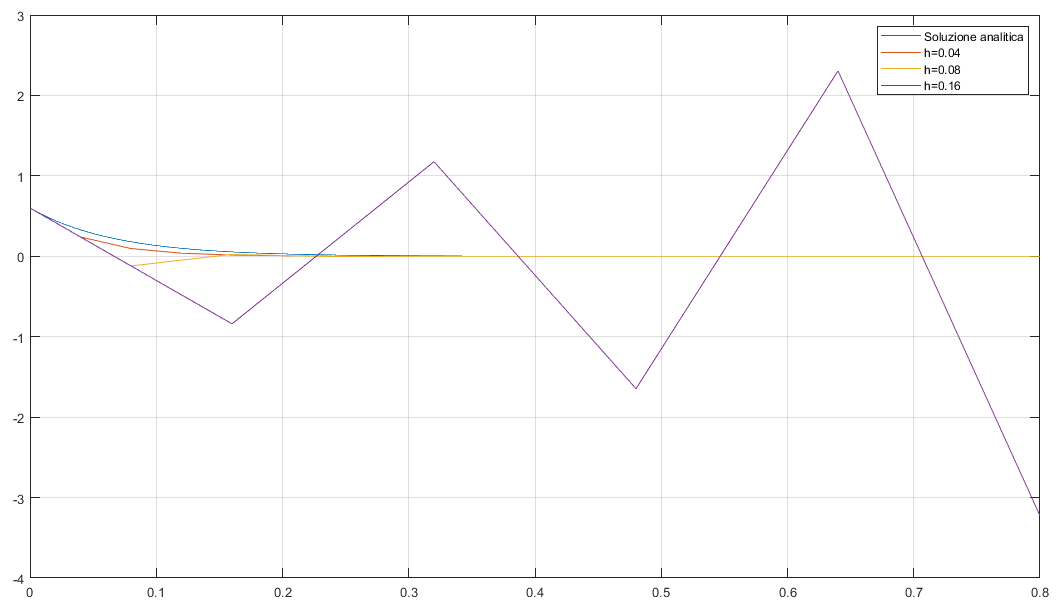
\includegraphics[width=\textwidth]{matlab/stabilita.png}
		\caption{\textit{Soluzione calcolata con h=0.04, h=0.08, h=0.16}}
	\end{figure}
	Quindi con $h=0.16$ la soluzione è del tutto inaccettabile, rendendo il metodo di Eulero un metodo per niente accurato.
\end{example}
LA stabilità di un metodo è data dal fatto che esso stesso non deve propagare un errore iniziale durante le successive iterazioni.
\\Sia $M_h(P)$ un problema discreto e $M^e_h(P)$ lo stesso problema discretto con un errore sul dato iniziale:
\begin{equation*}
	M_h(P) :
	\begin{cases}
		\dfrac{u(t_{i+1})-u(t_i)}{h} = f(t_i,u(t_i))  \\[0.2cm]
		u(t_{0}) = y(t_0)
	\end{cases}
	\qquad \forall i = \{0,1,...,n-1\}
\end{equation*}
e perturbando il problema con un errore $\epsilon_0$:
\begin{equation*}
	M^e_h(P) :
	\begin{cases}
		\dfrac{v(t_{i+1})-v(t_i)}{h} = f(t_i,v(t_i))  \\[0.2cm]
		v(t_{0}) = y(t_0)+\epsilon_0 = v_0
	\end{cases}
	\qquad \forall i = \{0,1,...,n-1\}
\end{equation*}
l'\textbf{errore di propagazione} al passo $i-esimo$ viene calcolato come:
\begin{equation}
	\epsilon_i(h) = v(t_i) - u(t_i)
\end{equation}
Partendo da questo calcolo si può definire la stabilità assoluta.


\subsection{Stabilità assoluta}
Siano $u(t_i)$ e $v(t_i)$ le soluzioni determinate con un metodo per la risoluzione di un problema ai valori iniziali rispettivamente ai dati iniziali $y_0$ e $v_0$, il metodo utilizzato si dice \textbf{assolutamente stabile} per un dato valore di $h$ se:
\begin{equation*}
	|\epsilon_0| \leq C \qquad \Rightarrow \qquad |\epsilon_i(h)| \leq C \quad \forall i \in \{0,1,...,n-1\}
\end{equation*}
con $C$ costante (upper bound).
\\Intuitivamente significa che l'errore in ogni intervallo di calcolo soddisfa la stessa limitazione dell'errore iniziale in tutto l'intervallo $[t_0, +\infty]$.

\subsection{Indice di condizionamento}
In riferimento dell'esempio precedente si intuisce che il valore di $h$ incide molto sulla soluzione. 
Il sistema di calcolo è un sistema aritmetico a precisione finita, quindi è importante dare una stima dell'indice di condizionamento. Se si riesce a trovare una funzione $g_i$ tale che associa al dato iniziale $y_0$ il valore della soluzione del problema discreto $M_h(P)$ allora:
\begin{equation*}
	C_A(g_i,y_0) = |g_i'(y_0)|
\end{equation*}
corrisponde all'indice di condizionamento assoluto.
\\Sulla base di ciò dato un problema di test come il seguente:
\begin{equation}
	\label{test}
	\begin{cases}
		\dfrac{dy}{dt} = \lambda y(t) \\[0.2cm]
		y(t_{0}) = y_0
	\end{cases}
\end{equation}
Per la legge di aggiornamento di Eulero si ha:
\begin{equation*}
	y_{i+1} = y_i + hf(t_i,y_i) \quad con \quad f(t_i,y_i) = \lambda y_i 
\end{equation*}
\begin{equation*}
	y_{i+1} = y_i + h\lambda y_i = (1+h\lambda)y_i = (1+h\lambda)^2y_{i-1} = ... = (1+h\lambda)^iy_0
\end{equation*}
quindi la funzione per calcolare l'indice di condizionamento del problema vale:
\begin{equation}
	\label{index_cond}
	g_i(y_0) = (1+h\lambda)^iy_0
\end{equation}
\begin{prop}[Condizionamento]
	Il metodo di Eulero è ben condizionato se e solo se:
	\begin{equation}
		\label{indice}
		\lambda = 0 \qquad opp. \qquad \left( \lambda<0 \; \wedge \; h < -\dfrac{2}{\lambda}\right)
	\end{equation}
\end{prop}
\textit{Dimostrazione.} Indicata con $g_i(y_0)$ la funzione che al dato iniziale $y_0$ associa il valore della soluzione $y_i$ del problema discreto, relativo al problema test \ref{test}, nel punto $t_i$, si ha per la \ref{index_cond}:
\begin{equation*}
	g_i(y_0) = y_i = (1+h\lambda)^i y_0
\end{equation*}
L'indice di condizionamento assoluto vale quindi:
\begin{equation*}
	C_A(g_i,y_0) = |g_i'(y_0)| = |(1+h\lambda)^i|
\end{equation*}
Il problema è ben condizionato se:
\begin{equation*}
	|(1+h\lambda)|^i \leq 1
\end{equation*}
Dato che $i\in \mathbb{N}$ allora:
\begin{equation*}
	|(1+h\lambda)| \leq 1 \quad \Rightarrow \quad -1 \leq (1+h\lambda) \leq 1
\end{equation*}
quindi, valutando le tre possibili situazioni:
\begin{itemize}
	\item \textbf{$\lambda$=0} Il problema è ben condizionato.
	\item \textbf{$\lambda$>0} L'equazione non ammette soluzioni accettabili, poiché richiede che $h$ sia negativo:
	\begin{equation*}
		|(1+h\lambda)| \leq 1 \quad \Rightarrow \quad (1+h\lambda) \leq 1 \quad \Rightarrow \quad h\leq 0
	\end{equation*}
	quindi il problema è sempre mal condizionato per qualunque $h$.
	\item \textbf{$\lambda$<0} Il problema è ben condizionato solo per alcuni valori di $h$:
	\begin{equation*}
		|(1+h\lambda)| \leq 1 \quad \Rightarrow \quad |(1-h|\lambda|)| \leq 1 \quad \Rightarrow \quad 
		-\dfrac{2}{|\lambda|} \leq -h \leq 0 \quad \Rightarrow \quad   0\leq h \leq \dfrac{2}{|\lambda|}
	\end{equation*}
	Si ha dunque la tesi.
\end{itemize}

\begin{example}
	Riprendendo quindi l'esempio precedente, la divergenza si aveva per:
	\begin{equation*}
		h=0.16 \qquad \lambda = -15
	\end{equation*}
	Questo perchè l'indice di condizionamento è maggiore di 1, andando ad amplificare l'errore, infatti:
	\begin{equation*}
		\dfrac{2}{|\lambda|}= \dfrac{2}{15} = 0.1\bar{3} < 0.16 = h
	\end{equation*}
Dunque il problema era mal condizionato. Per gli altri valori di $h$ invece era ben condizionato.
\end{example}

\subsection{Zero-Stabilità}
A differenza della stabilità assoluta, che studia l'andamento della soluzione con $h$ prefissato e in un intervallo $[t_0, +\infty]$, la zero-stabilità studia la soluzione numerica nell'intervallo $[t_0, T]$ con $h\rightarrow 0$.
Un metodo di risoluzione a step è \textbf{zero-stabile} se esistono $h_0>0$ e $K>0$ tali che:
\begin{equation*}
	|\epsilon_i(h)| \leq K|\epsilon_0| \quad per\quad  h\leq h_0
\end{equation*}
\\Il metodo di Eulero è zero-stabile poiché:
\begin{equation*}
	|\epsilon_i(h)| \leq e^{(T-t_0)L}|\epsilon_0| \quad con \quad e^{(T-t_0)L}=K
\end{equation*}
La zero-stabilità dipende inoltre dall'errore iniziale $\epsilon_0$. La propagazione si può mantenere sotto ad una determinata soglia se $\epsilon_0$ è "sufficientemente piccolo".

\begin{theorem}[Teorema di Lax-Dahlquist]
Un metodo numerico è consistente e zero-stabile se e solo se è convergente. Vale il viceversa.
\\Inoltre l'ordine di consistenza coincide con l'ordine di convergenza.
\end{theorem}
Il teorema sopra citato è molto importante. Attraverso la conoscenza di stabilità e consistenza, parametri più semplici da calcolare, si possono ricavare informazioni sulla convergenza, parametro invece più difficile da calcolare.
\section{Esempio semplice}
Si consideri il seguente problema in $t=[0,1]$:
\begin{equation*}
	\begin{cases}
		\dfrac{dy}{dt} = -10y(t) \\[0.2cm]
		y(t_{0}) = 1
	\end{cases}
\end{equation*}
La soluzione analitica è conosciuta e vale:
\begin{equation*}
	y(t) = e^{-10t}
\end{equation*}

\subsection{Stabilità}
In prima analisi bisogna fissare un passo di discretizzazione $h$ (o il numero di intervalli $N$) limite, in modo da mantenersi in una regione di stabilità. Per la \ref{indice} si ha:
\begin{equation*}
	h < \dfrac{2}{10} = 0.2
\end{equation*}
oppure:
\begin{equation*}
	h = \dfrac{T-t_0}{N} \quad \Rightarrow \quad N = \dfrac{T-t_0}{h} > \dfrac{1}{0.2} > 5
\end{equation*}
Eseguendo il seguente script infatti (per N=5 e N=20):
\begin{minted}[framesep = 1mm,
	fontsize = \footnotesize,
	]{MATLAB}
	lambda = -10;
	
	f = @(t,y) lambda*y;  %Soluzione y(t) = e^(lambda*t)
	N = [5 10^7];         %Numero di iterazioni
	t0 = 0; T=1; y0=1;    %Condizioni iniziali 
	h=(T-t0)./N;          %Passo di discretizzazione
	
	t = t0:h(end):T;     %Asse dei tempi per la soluzione analitica
	y_analitica = exp(lambda.*t);
	plot(t,y_analitica,'LineWidth', 2, 'Color', 'black');
	hold on;
	
	t = t0:h(1):T;       %Asse dei tempi
	y_numerica = eulero32(f, y0, t0, T, h(1));
	plot(t,y_numerica, 'LineWidth', 2);
	xlabel('Tempo');
	ylabel('Soluzione');
	legend('Soluzione Analitica', 'h=5');
	grid;
\end{minted}
\begin{figure}[H]
	\centering   
	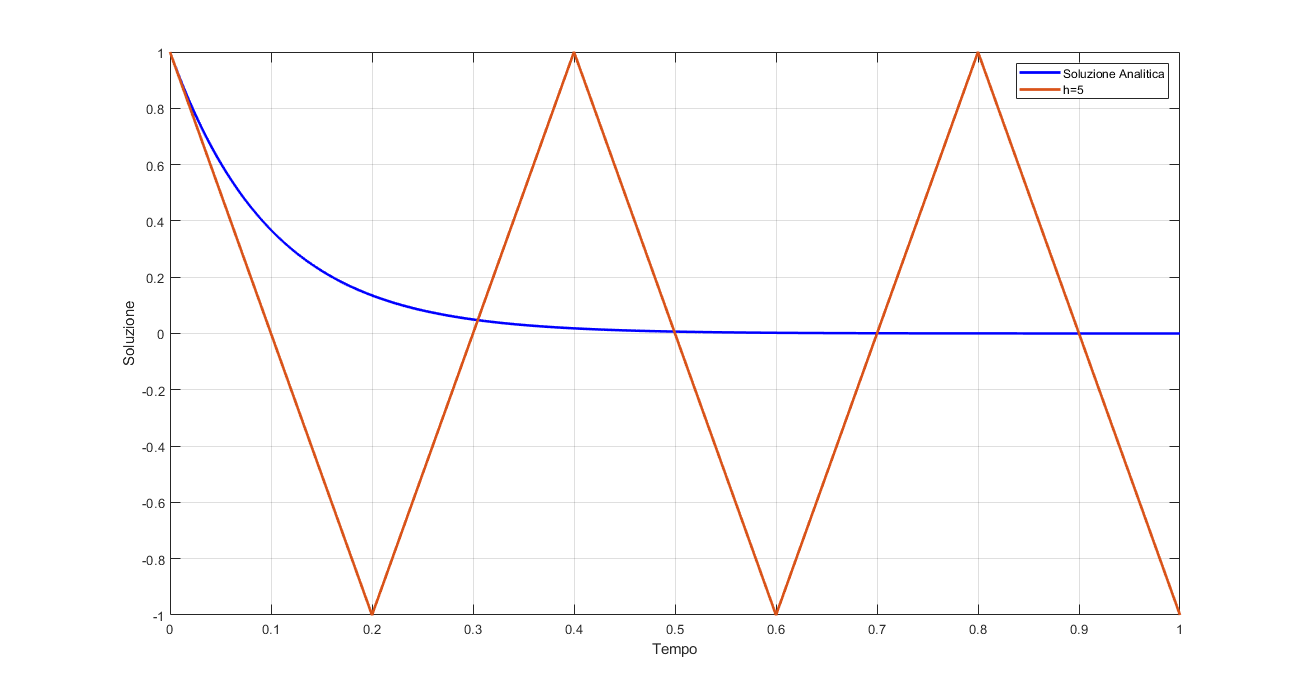
\includegraphics[width=\textwidth]{matlab/esercizio1_stabilita.png}
	\caption{\textit{N=5}}
\end{figure}
\begin{figure}[H]
	\centering   
	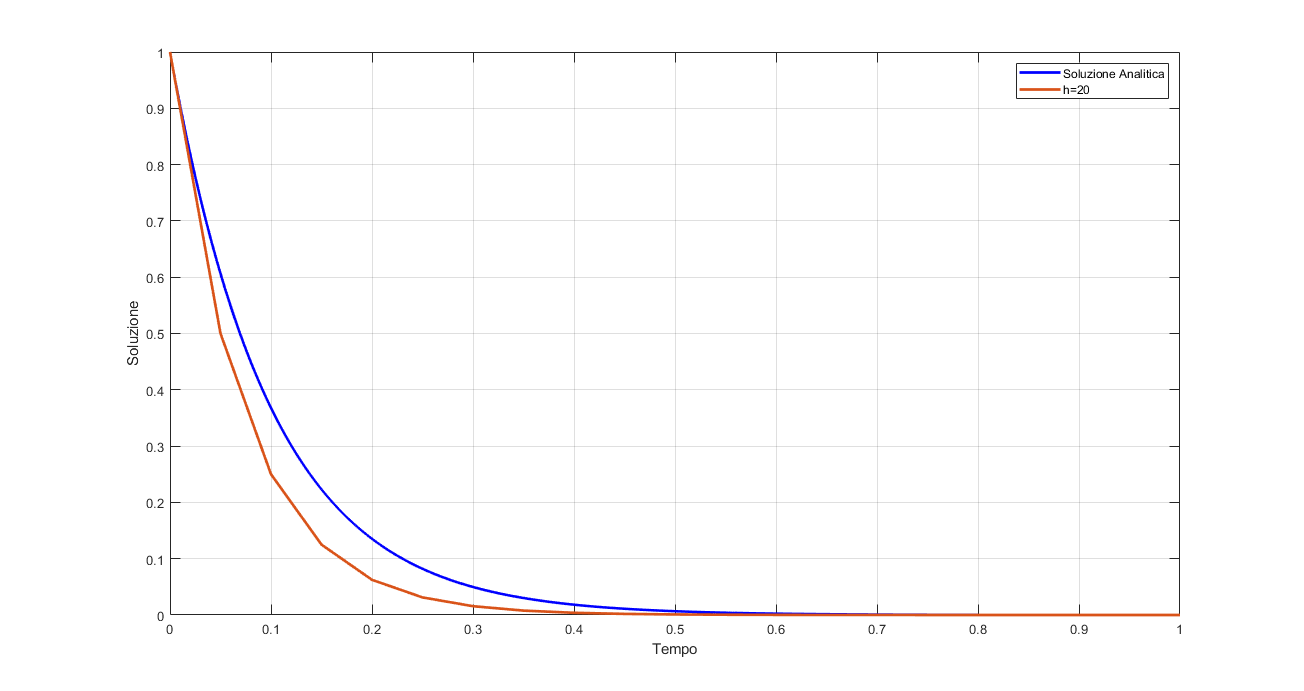
\includegraphics[width=\textwidth]{matlab/esercizio1_stabilita2.png}
	\caption{\textit{N=20}}
\end{figure}

\subsection{Errore Totale}
L'errore totale prevede una componente di \textit{errore di troncamento globale} (diminuisce al crescere di $N$) e una componente di \textit{errore di roundoff} (aumenta al crescere di $N$). Per dare una visione grafica di quest'errore si sono calcolate varie soluzioni numeriche con diversi valori di $N$.
\begin{minted}[framesep = 1mm,
	fontsize = \footnotesize,
	]{MATLAB}
	lambda = -10;
	
	f = @(t,y) lambda*y;    %Soluzione y(t) = e^(lambda*t)
	N = [10^2 10^3 10^4 10^5 10^6 10^7];          
	t0 = 0; T=1; y0=1; 
	h=(T-t0)./N;            
	
	e_tot = zeros(1,length(N));
	t = t0:h(end):T;
	y_analitica = exp(lambda.*t);
	plot(t,y_analitica,'LineWidth', 2, 'Color', 'blue');
	
	hold on;
	for i=1:length(N)
	t = t0:h(i):T; 
	y_numerica = eulero32(f, y0, t0, T, h(i)));
	e_tot(i) = abs(y_numerica(end)-y_analitica(end));
	plot(t,y_numerica, 'LineWidth', 2);
	end
	
	xlabel('Tempo');
	ylabel('Soluzione');
	legend('Soluzione Analitica','h=10^2', 'h=10^3', 'h=10^4','h=10^5','h=10^6','h=10^7');
	grid;
\end{minted}
\begin{figure}[H]
	\centering   
	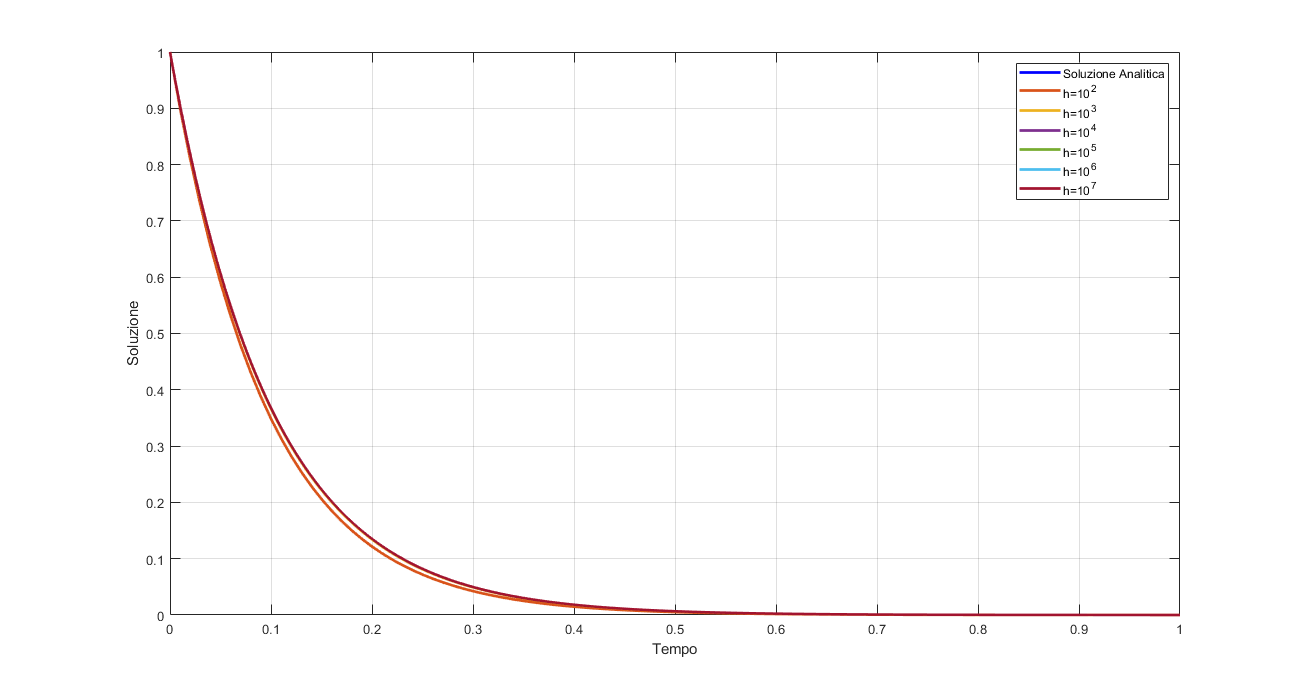
\includegraphics[width=\textwidth]{matlab/esercizio1_soluzioni.png}
	\caption{\textit{Grafico di tutte le soluzioni numeriche calcolate}}
\end{figure}
Si può effettuare uno zoom sulle curve per vedere meglio i confronti:
\begin{figure}[H]
	\centering   
	\subfigure{	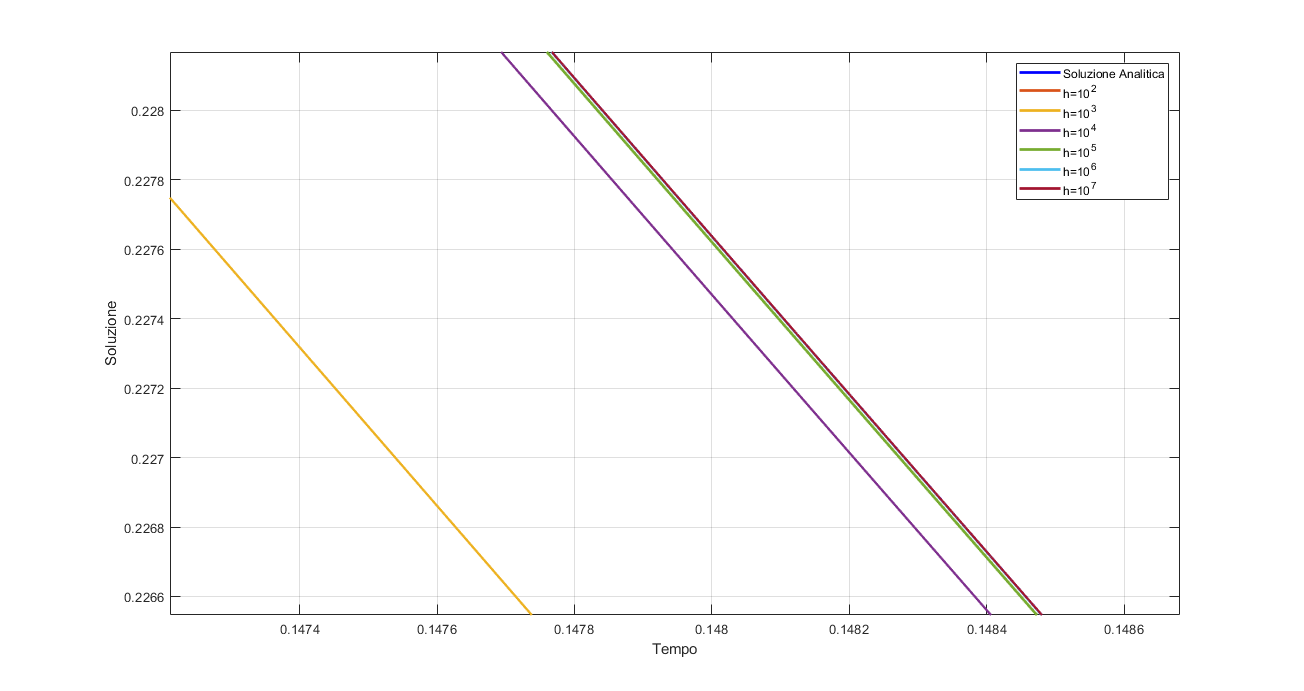
\includegraphics[width=0.45\textwidth]{matlab/esercizio1_soluzioni_zoom1.png}}
	\subfigure{	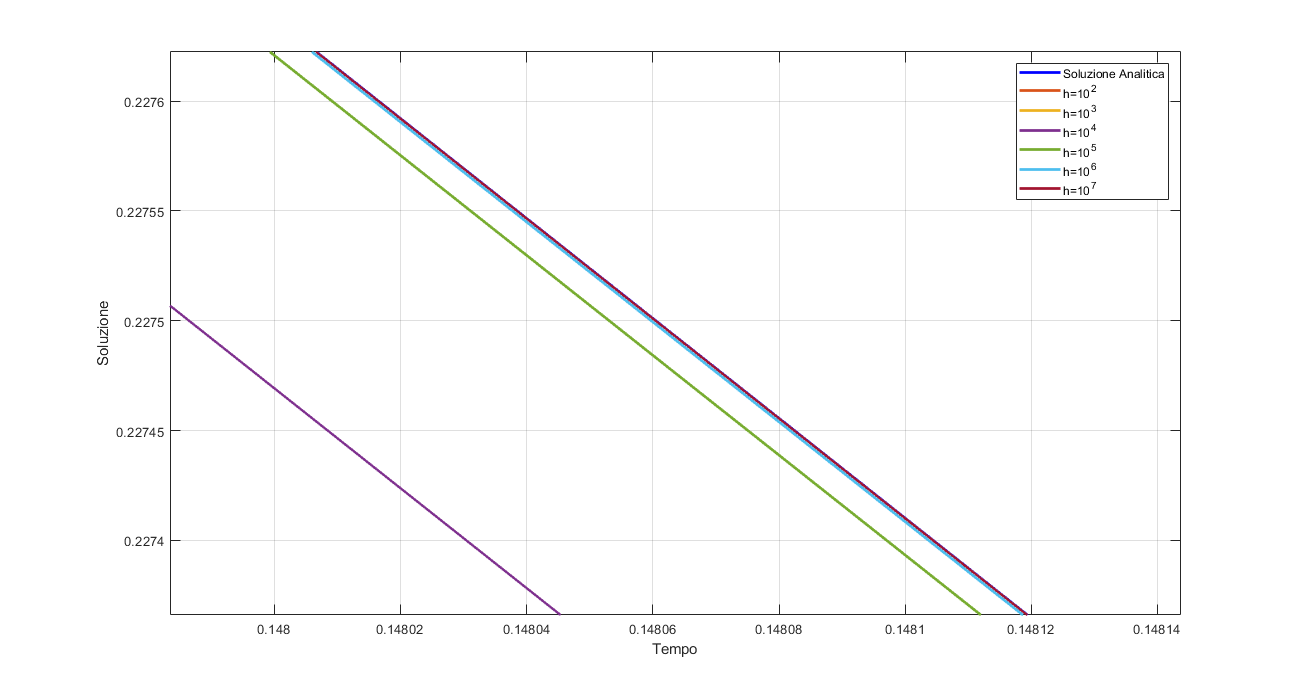
\includegraphics[width=0.45\textwidth]{matlab/esercizio1_soluzioni_zoom2.png}}	
	\subfigure{	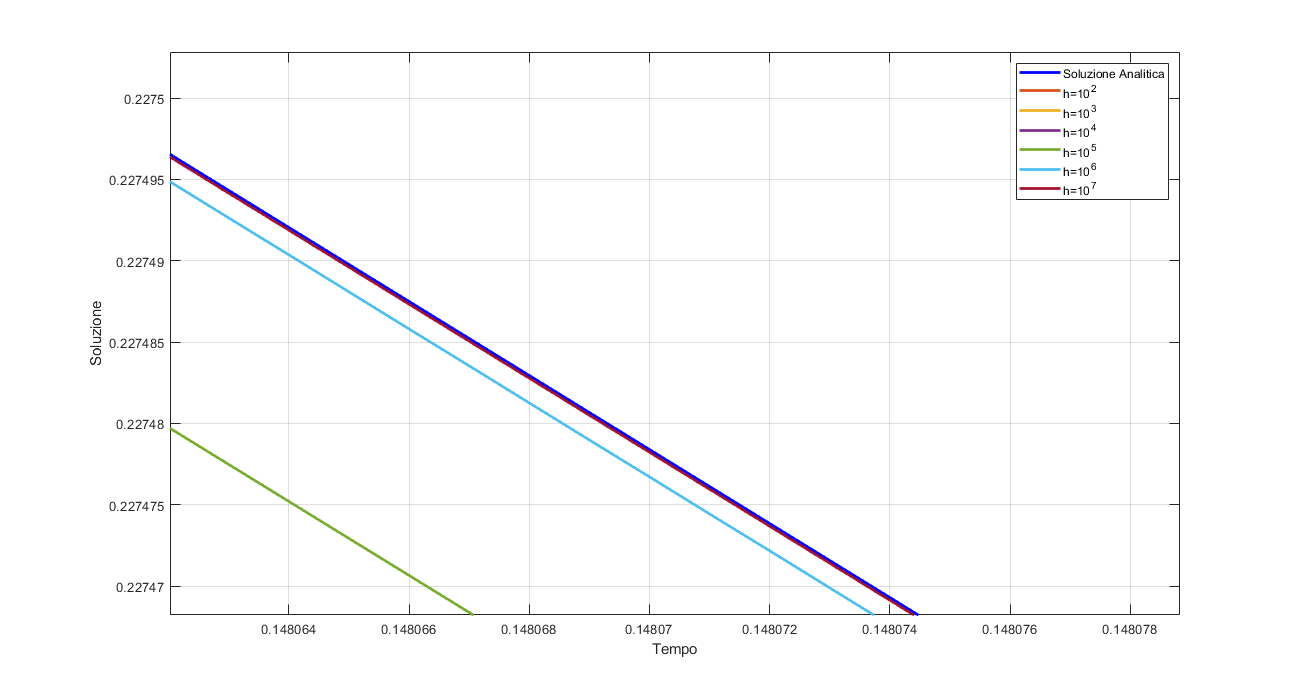
\includegraphics[width=0.45\textwidth]{matlab/esercizio1_soluzioni_zoom3.png}}
	\subfigure{	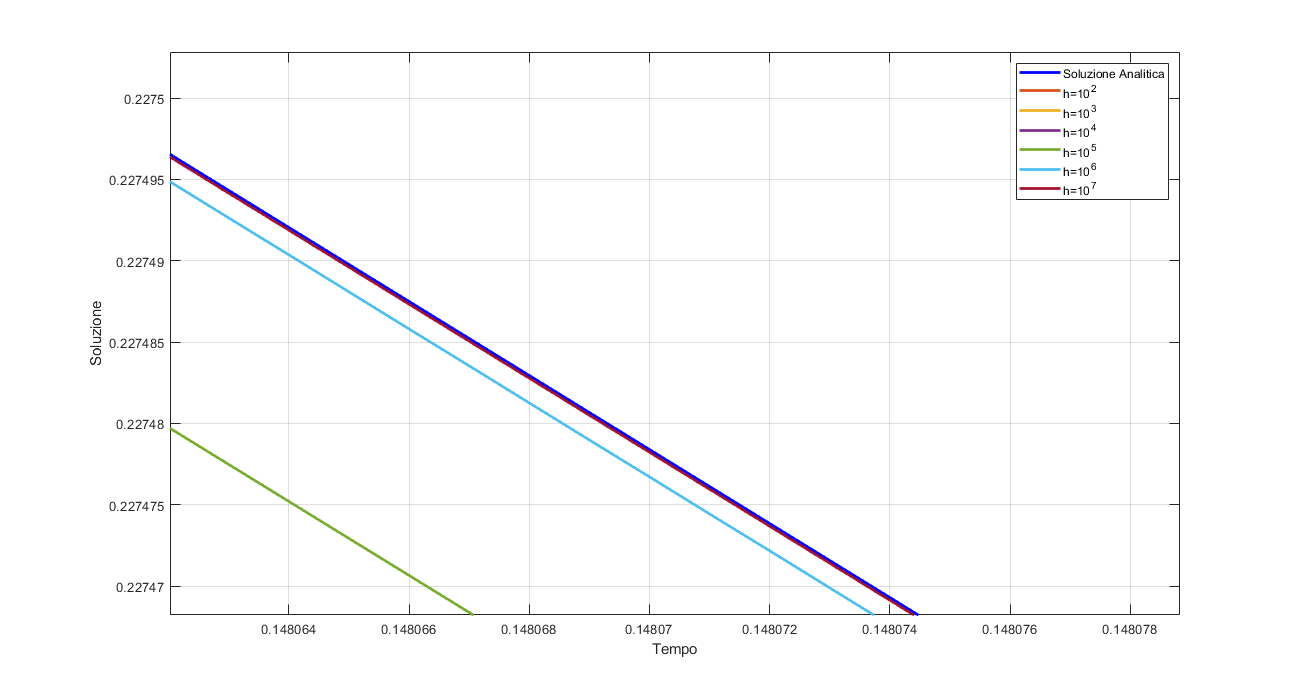
\includegraphics[width=0.45\textwidth]{matlab/esercizio1_soluzioni_zoom4.png}}
	\caption{\textit{Zoom del grafico in corrispondenza delle varie curve}}
\end{figure}
A questo punto si può studiare l'andamento dell'errore. Esso si propaga fino all'ultimo step. Per ogni curva numerica quindi si può calcolare l'errore totale come:
\begin{equation*}
	e_{tot} = |y_{numerica}(end) - y_{analitica}(end)|
\end{equation*}
Dato che l'interesse è sull'ordine di grandezza, il grafico può essere fatto in scala logaritmica. A partire dallo script precedente quindi:
\begin{minted}[framesep = 1mm,
	fontsize = \footnotesize,
	]{MATLAB}
	loglog(N, e_tot,'LineWidth',2);
	hold on;
	loglog(N, e_tot, '+');
	grid;
\end{minted}
\begin{figure}[H]
	\centering   
	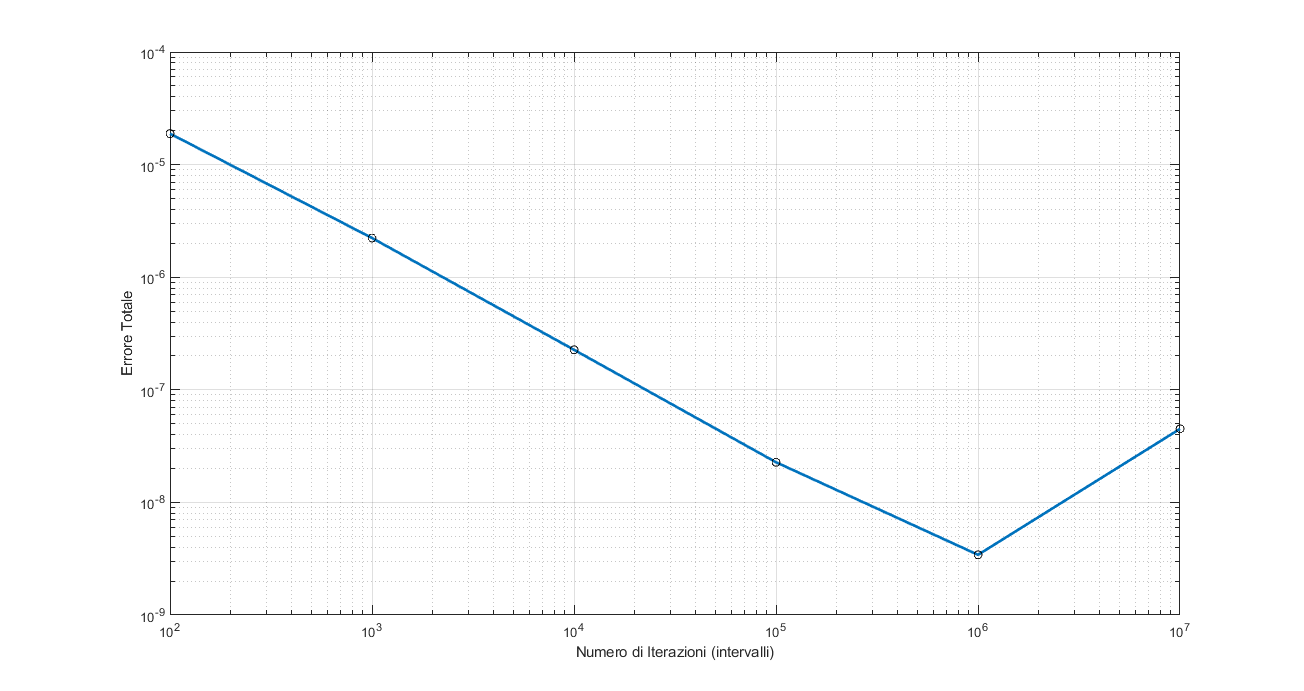
\includegraphics[width=\textwidth]{matlab/esercizio1_errore_totale.png}
	\caption{\textit{Errore calcolato sull'ultima componente di ogni soluzione numerica rispetto alla soluzione analitica}}
\end{figure}
Nella figura si notato due andamenti diversi:
\begin{enumerate}
	\item $N<10^5$ si ha un andamento proporzionale a $O(h)$. Questo perché per valori piccoli di $N$ (e grandi di $h$) prevale l'errore di troncamento invece dell'errore di roundoff.
	\item $N>10^5$ si inizia a perdere la linearità e si ha un'andamento in cui l'errore inizia a crescere, ciò significa che l'errore di roundoff prevale sull'errore di troncamento, poiché si tratta di valori di $N$ molto grandi (e piccoli di $h$).
\end{enumerate}

\subsubsection{Errore di Troncamento Globale}
Le soluzioni numeriche calcolate in precedenza sono state calcolate utilizzando una rappresentazione in \textit{singola precisione}. 
\\Per ricavare il contributo dell'errore di troncamento si può assumere che la soluzione in \textit{doppia precisione} sia la soluzione numerica corretta, ovvero senza errore di roundoff.
\\Quindi l'errore vale:
\begin{equation*}
	gte = |y_{numerica\_double}(end) - y_{analitica}(end)|
\end{equation*}
Dato che si propaga, basta considerare l'ultimo elemento del vettore soluzione.
\begin{minted}[framesep = 1mm,
	fontsize = \footnotesize,
	]{MATLAB}
	gte = zeros(1,length(N));
	e_tot = zeros(1, length(N));
	t = t0:h(end):T;
	y_analitica = exp(lambda.*t);
	
	hold on;
	for i=1:length(N)
	t = t0:h(i):T;  %Asse dei tempi
	y_numerica = eulero32(f, y0, t0, T, h(i));
	y_numerica_double = eulero64(f, y0, t0, T, h(i));
	e_tot(i) = abs(y_analitica(end)-y_numerica(end));
	gte(i) = abs(y_analitica(end)-y_numerica_double(end));
	end
	
	figure;
	p1 = loglog(N, e_tot, 'LineWidth', 2);
	hold on;
	loglog(N, e_tot, 'o', 'Color', 'Black');
	p2 = loglog(N, gte, '--', 'Color', 'Red', 'LineWidth', 2);
	xlabel('Numero di Iterazioni (intervalli)');
	ylabel('Errore Totale');
	legend([p1 p2], {'Errore Totale', 'GTE'});
\end{minted}
\begin{figure}[H]
	\centering   
	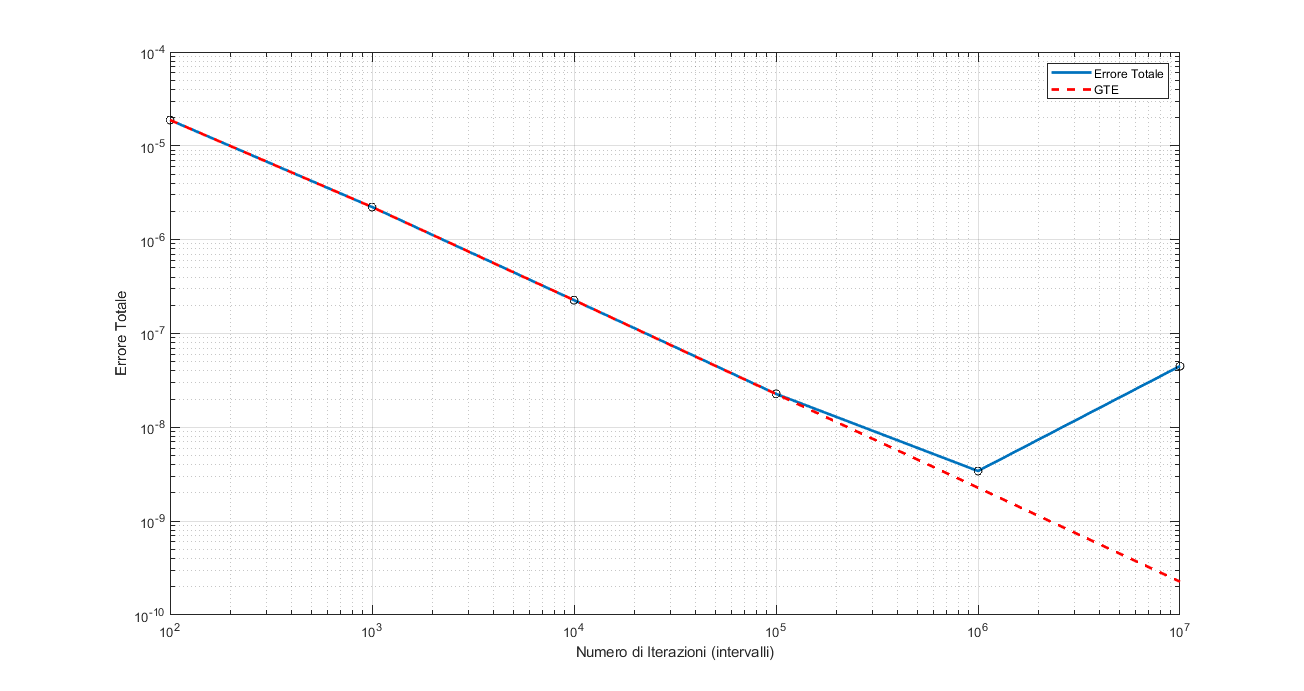
\includegraphics[width=\textwidth]{matlab/esercizio1_errore_troncamento.png}
	\caption{\textit{Errore di troncamento calcolato sull'ultima componente di ogni soluzione numerica rispetto alla soluzione analitica}}
\end{figure}

\subsubsection{Errore di Round-Off}
Allo stesso modo si può calcolare l'errore di roundoff come differenza tra la soluzione in \textit{singola precisione} e in \textit{doppia precisione}:
\begin{equation*}
	roundoff = |y_{numerica\_double}(end) - y_{numerica}(end)|
\end{equation*}
\begin{minted}[framesep = 1mm,
	fontsize = \footnotesize,
	]{MATLAB}
	gte = zeros(1,length(N));
	e_tot = zeros(1, length(N));
	roundoff = zeros(1,length(N));
	t = t0:h(end):T;
	y_analitica = exp(lambda.*t);
	
	hold on;
	for i=1:length(N)
	t = t0:h(i):T;  %Asse dei tempi
	y_numerica = eulero32(f, y0, t0, T, h(i));
	y_numerica_double = eulero64(f, y0, t0, T, h(i));
	e_tot(i) = abs(y_analitica(end)-y_numerica(end));
	gte(i) = abs(y_analitica(end)-y_numerica_double(end));
	roundoff(i) = abs(y_numerica(end) - y_numerica_double(end));
	end
	
	figure;
	p1 = loglog(N, e_tot, 'LineWidth', 2);
	hold on;
	loglog(N, e_tot, 'o', 'Color', 'Black');
	p2 = loglog(N, gte, '--', 'Color', 'Red', 'LineWidth', 2);
	p3 = loglog(N, roundoff, '--','Color', 'Black', 'LineWidth', 2);
	xlabel('Numero di Iterazioni (intervalli)');
	ylabel('Errore Totale');
	legend([p1 p2 p3], {'Errore Totale', 'GTE', 'RoundOff'});
\end{minted}
\begin{figure}[H]
	\centering   
	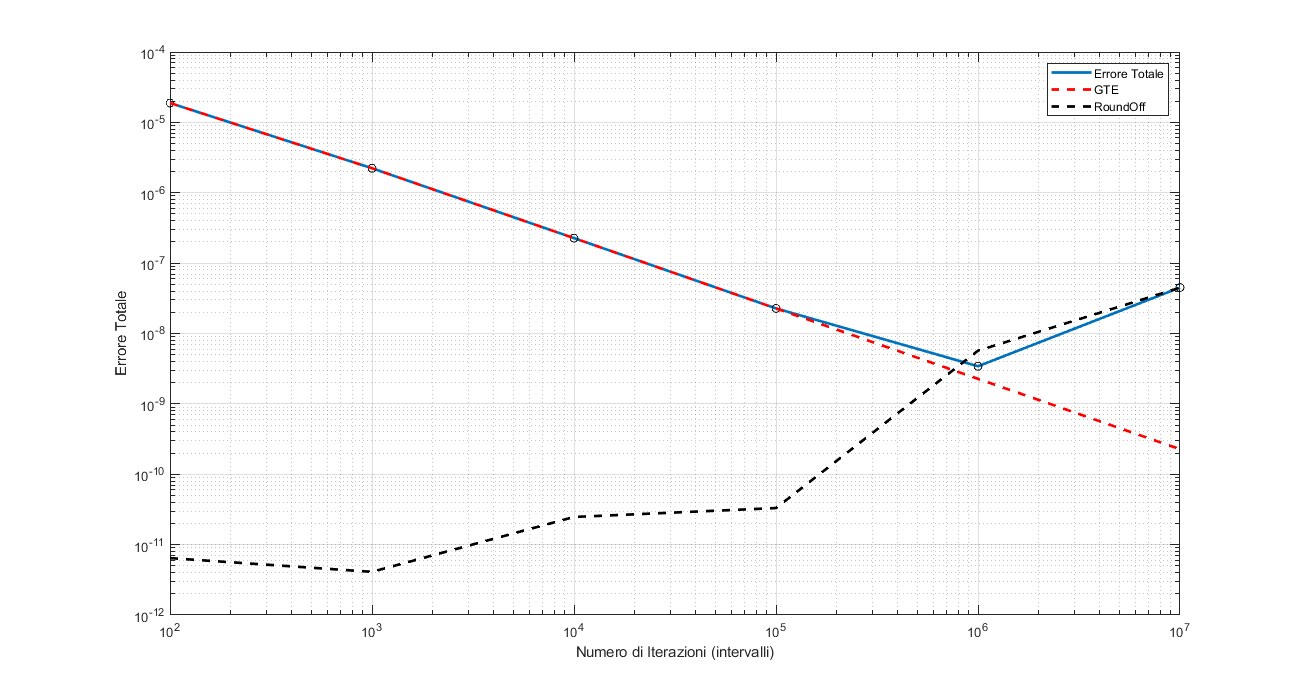
\includegraphics[width=\textwidth]{matlab/esercizio1_errore_roundoff.png}
	\caption{\textit{Errore di roundoff calcolato sull'ultima componente di ogni soluzione numerica}}
\end{figure}
Nell'estremo destro del grafico si può notare come la curva dell'errore di roundoff diventa dominante nel errore totale.
\\Per verificare l'equazione \ref{e_tot} si può aggiungere al grafico la somma dell'errore di roundoff e l'errore di troncamento globale calcolato in precedenza.
\begin{figure}[H]
	\centering   
	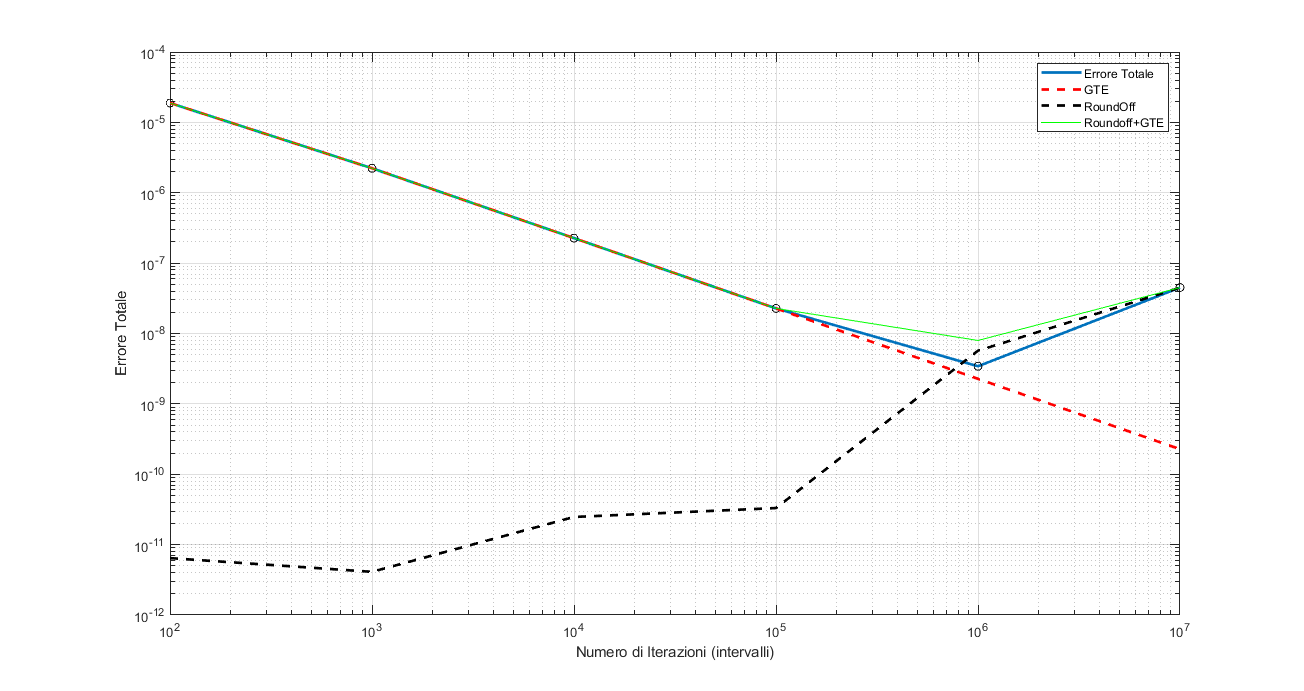
\includegraphics[width=\textwidth]{matlab/esercizio1_errore_somma.png}
	\caption{\textit{Grafico degli errori calcolati}}
\end{figure}
Si nota quindi che:
\begin{equation*}
	e_{tot} < |roundoff| + |gte|
\end{equation*}
\subsection{Numero di intervalli ottimo}
Per avere una visione più chiara di ciò che succede intorno a $10^6$, si possono calcolare le soluzioni e gli errori in tale intorno:
\begin{figure}[H]
	\centering   
	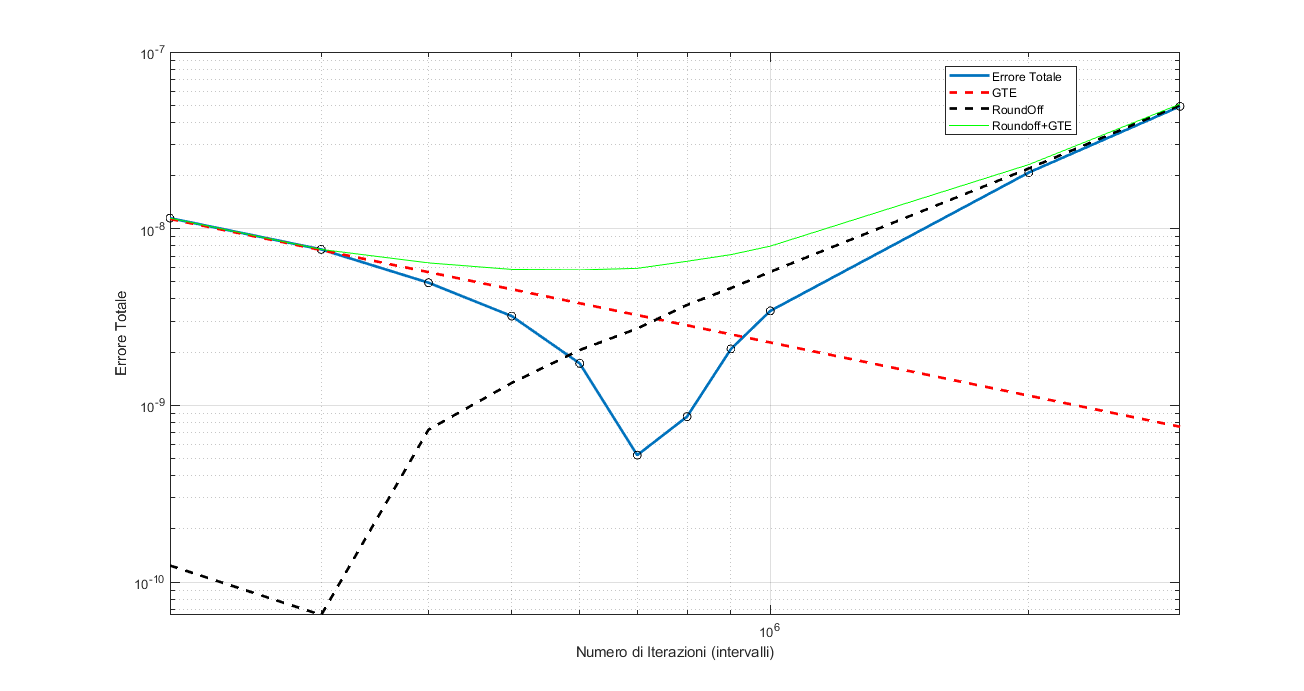
\includegraphics[width=\textwidth]{matlab/esercizio1_errore_confronto.png}
	\caption{\textit{Grafico degli errori calcolati}}
\end{figure}
In verde si è messo in risalto la funzione maggiorata dell'errore totale, molto simile alla funzione descritta in Fig.\ref{e_tot_fig}.\\
Il valore ottimo di $N$ (e di $h$) equivale all'incrocio delle due curve degli errori, poiché si ottiene la massima accuratezza.
\begin{equation*}
	N_{opt} \approx 7.2\times10^5 \qquad h_{opt} \approx 0.138\times 10^{-5}
\end{equation*}
L'errore minimo che si commette è di circa $10^{-9}$.
\\Se l'errore non è accettabile nel contesto in cui viene calcolata la soluzione, allora il metodo di Eulero non è il metodo più adatto. In tal caso bisogna affidarsi a metodi più precisi.

	\chapter{Applicazioni}
\section{Sistemi di Equazioni Differenziali}
Fin ora sono stati tratti solo problemi di Cauchy del primo ordine, del tipo \ref{ode}. Il più delle volte però si è costretti ad analizzare equazioni differenziali di ordine superiore al primo:
\begin{equation}
	y^n(t) = f(t, y(t), y'(t), y''(t),...,y^{n-1}(t))
\end{equation}
con $n-1$ condizioni iniziali.
\\Introducendo delle variabili ausiliarie:
\begin{equation*}
	z_1(t) = y(t) \quad z_2(t) = y'(t) \quad ... \quad z_N(t) = y^{n-1}(t)
\end{equation*}
si può ottenere una equazione differenziale del primo ordine equivalente:
\begin{equation*}
	\textbf{z}'(t) = \begin{pmatrix}
		z_1'(t) \\ z_2'(t) \\ \vdots \\ z_n'(t)
	\end{pmatrix}
 	= \begin{pmatrix}
 		y'(t) \\ y''(t) \\ \vdots \\ y^{n}(t)
 	\end{pmatrix}
 	= \begin{pmatrix}
 		z_2(t) \\ z_3(t) \\ \vdots \\ f(t, z_1(t), z_2(t), ..., z_n(t))
 	\end{pmatrix}
 	= \textbf{g}(t, \textbf{z}(t))
\end{equation*}
A questo punto si può applicare il metodo di Eulero alla variabile $\textbf{z}(t)$ multidimensionale.
\begin{example}
	Sia il seguente problema di Cauchy:
	\begin{equation*}
		x''(t) = -\lambda x(t)
	\end{equation*}
	con $x(0) = 0$ e $x'(0) = 0$
	Utilizzando $\textbf{v}(t)$ come variabile ausiliaria:
	\begin{equation*}
		\textbf{v}(t) = \begin{pmatrix}
			x(t) \\ x'(t)
		\end{pmatrix}
		= \begin{pmatrix}
			v_1(t) \\ v_2(t)
		\end{pmatrix}
	\end{equation*}
	La nuova equazione differenziale diventa:
	\begin{equation*}
		\textbf{v}'(t) = \begin{pmatrix}
			x'(t) \\ x''(t)
		\end{pmatrix}
		= \begin{pmatrix}
			v_2(t) \\ -\lambda v_1(t)
		\end{pmatrix}
	 	= \textbf{g}(t, \textbf{v}(t))
	\end{equation*}
	in cui $\textbf{g}(t)$ è la nuova funzione vettoriale che descrive $\textbf{v}'(t)$
\end{example}
L'implementazione in MATLAB prevede un cambiamento rispetto alla normale implementazione descritta in precedenza.
\\I parametri di ingresso alla funzione sono:
\begin{itemize}
	\item \textbf{$f$} Funzione vettoriale dell'equazione differenziale di tipo \ref{ode}
	\item \textbf{$y_0$} Vettore delle condizioni iniziali al tempo $t_0$
	\item \textbf{$t_0$} Tempo iniziale
	\item \textbf{$T$} Tempo finale
	\item \textbf{$h$} Passo di discretizzazione
\end{itemize}
I parametri in uscita sono:
\begin{itemize}
	\item \textbf{$t$} Asse dei tempi discretizzato
	\item \textbf{$y$} Matrice soluzione soluzione
\end{itemize} 
La soluzione $y(t)$ viene vista come un vettore di vettori. Definito il passo di discretizzazione $h$ e, quindi, $N$ numero di intervalli, la dimensione della soluzione è $n\times N$ (con $n$ ordine dell'equazione differenziale).
\begin{minted}[framesep = 1mm,
	fontsize = \footnotesize,
	]{MATLAB}
function [y, t] = eulero32(f, y0, t0, T, h)
	t = single(t0:h:T);                 %Asse dei tempi discretizzata con passo h
	y = single(zeros(length(y0),length(t)));     %Vettore soluzione
	y(:,1) = y0;                  %Condizione iniziale
	
	for i=1:length(t)-1
		y(:,i+1) = y(:,i) + f(t(i), y(:,i))*h;    %Costruzione della soluzione
	end
end
\end{minted}
\begin{minted}[framesep = 1mm,
	fontsize = \footnotesize,
	]{MATLAB}
function [y, t] = eulero64(f, y0, t0, T, h)
	t = t0:h:T;                 %Asse dei tempi discretizzata con passo h
	y = zeros(zeros(length(y0),length(t));     %Vettore soluzione
	y(:,1) = y0;                  %Condizione iniziale
	
	for i=1:length(t)-1
		y(:,i+1) = y(:,i) + f(t(i), y(:,i))*h;    %Costruzione della soluzione
	end
end
\end{minted}
Il metodo di Eulero viene calcola insieme tutte le soluzioni. Ogni riga rappresenta un vettore soluzione.
\\Questa modifica rende il metodo di Eulero più generale. Infatti una equazione differenziale del primo ordine può essere vista come un sistema di equazioni vettoriali con una sola equazione.

\section{Sistema Massa-Molla}
Il sistema massa-molla è un sistema meccanico composto da un corpo di massa $m$, attaccato ad una molla con constante elastica $k$.
\begin{figure}[H]
	\centering   
	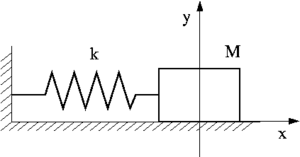
\includegraphics[width=0.5\textwidth]{img/massa-molla.png}
\end{figure} 
Il modello è descritto dalla seguente equazione differenziale:
\begin{equation*}
	m \dfrac{d^2x}{dt^2} = -kx	
\end{equation*}
La soluzione analitica è conosciuta e vale:
\begin{equation*}
	x(t) = A cos(\omega_0t) \quad con \quad \omega_0=\dfrac{k}{m}
\end{equation*}

A questo punto si hanno tutti gli strumenti per analizzare l'errore prodotto dal metodo di Eulero.
\\Si inizia con il calcolo della soluzione numerica per vari $N$:
\begin{minted}[framesep = 1mm,
	breaklines,
	fontsize = \footnotesize,
	]{MATLAB}
%Parametri
k=1;
m=1;

%Condizioni iniziali
t0=0; T=2;
x0=0; v0=1;
y0=[x0,v0];

%Passo di discretizzazione
N = [10^2 10^3 10^4 10^5 10^6 10^7];
h=(T-t0)./N;

%Soluzione anlitica
tempo = t0:h(end):T;
y_analitica = [sin(tempo); cos(tempo)];
plot(tempo, y_analitica(1,:), 'Color', 'Black', 'LineWidth',2);

%Inizializzazione degli errori
gte = zeros(1,length(N));
e_tot = zeros(1, length(N));
e_tot_equivalente = zeros(1, length(N));
roundoff = zeros(1,length(N));
plot(tempo,y_analitica(1,:));

%Soluzione numerica
hold on;
f = @(t,y) [y(2); -k/m*y(1)]; 
for i=1:length(N)
	t = t0:h(i):T;  %Asse dei tempi
	y_numerica = eulero32(f, y0, t0, T, h(i));
	y_numerica_double = eulero64(f, y0, t0, T, h(i));
	roundoff(i) = abs(y_numerica_double(1,end) - y_numerica(1,end));
	e_tot(i) = abs(y_analitica(1,end)-y_numerica(1,end));
	e_tot_equivalente(i) =  abs(y_numerica_double(1,end) - y_numerica(1,end) + y_analitica(1,end)-y_numerica_double(1,end));
	gte(i) = abs(y_analitica(1,end)-y_numerica_double(1,end));
	plot(t,y_numerica(1,:), 'LineWidth', 2);
end
legend('Soluzione Analitica', 'N=10^2', 'N=10^3','N=10^4', 'N=10^5', 'N=10^6', 'N=10^7');
xlabel('Tempo');
ylabel('Soluzione');
grid;
\end{minted}
L'output è il seguente:
\begin{figure}[H]
	\centering   
	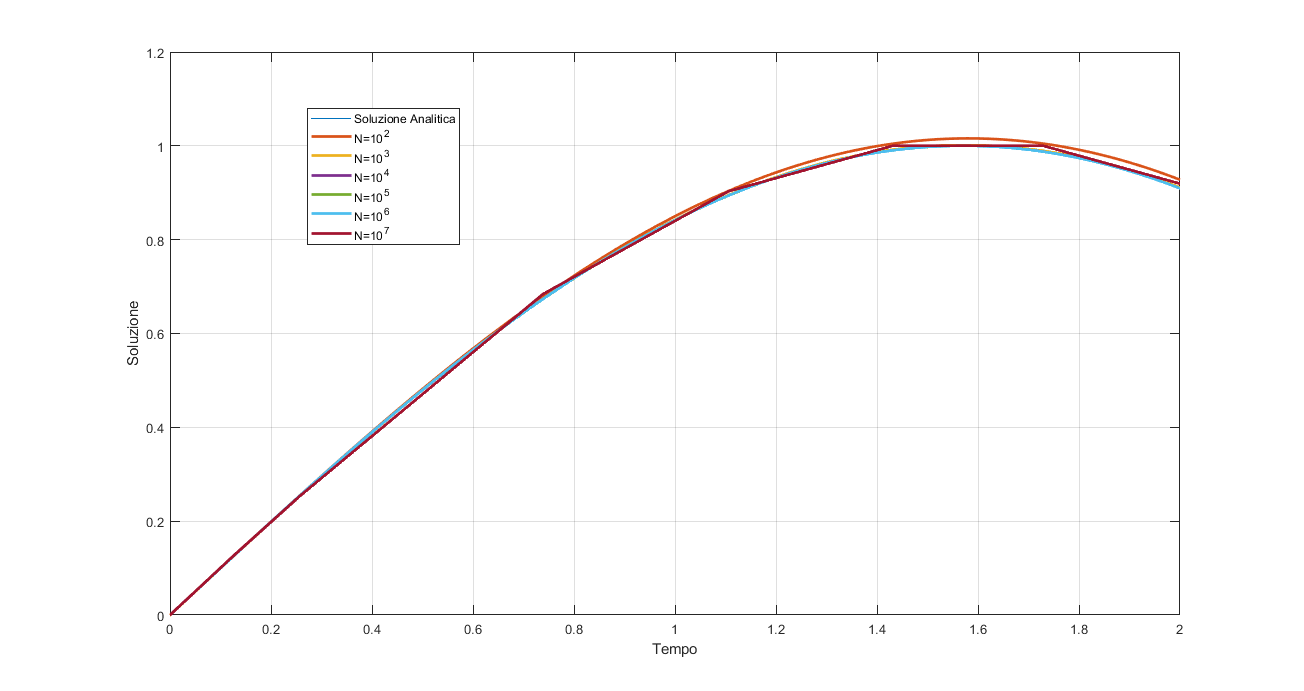
\includegraphics[width=\textwidth]{matlab/esercizio2_soluzioni.png}
	\caption{\textit{Confronto tra le varie soluzioni calcolate}}
\end{figure}
Effettuando uno zoom del grafico si possono notare delle particolarità.
\begin{figure}[H]
	\centering   
	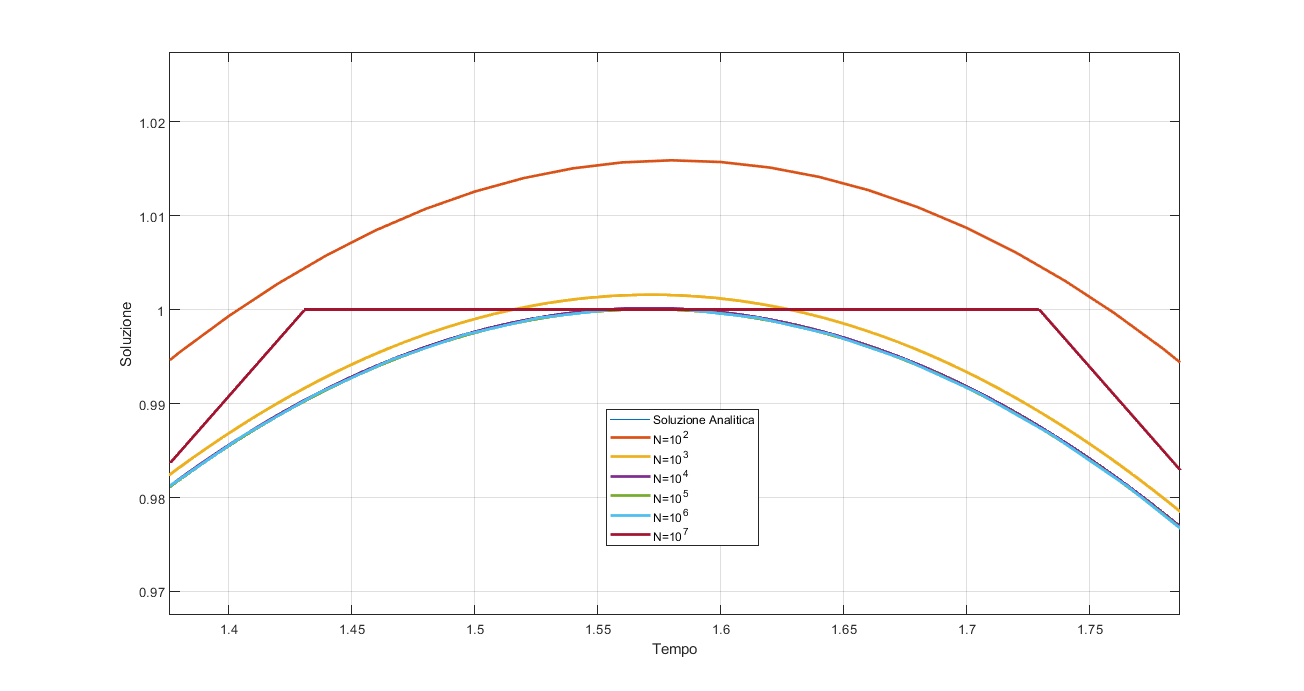
\includegraphics[width=\textwidth]{matlab/esercizio2_soluzioni_zoom1.png}
	\caption{\textit{Zoom delle soluzioni}}
\end{figure}
Già dal grafico si può notare l'influenza dell'errore di roundoff. Infatti per $N=10^7$ l'andamento della soluzione numerica è molto diverso rispetto all'andamento della soluzione analitica.
\\Andando ad effettuare l'analisi degli errori infatti:
\begin{figure}[H]
	\centering   
	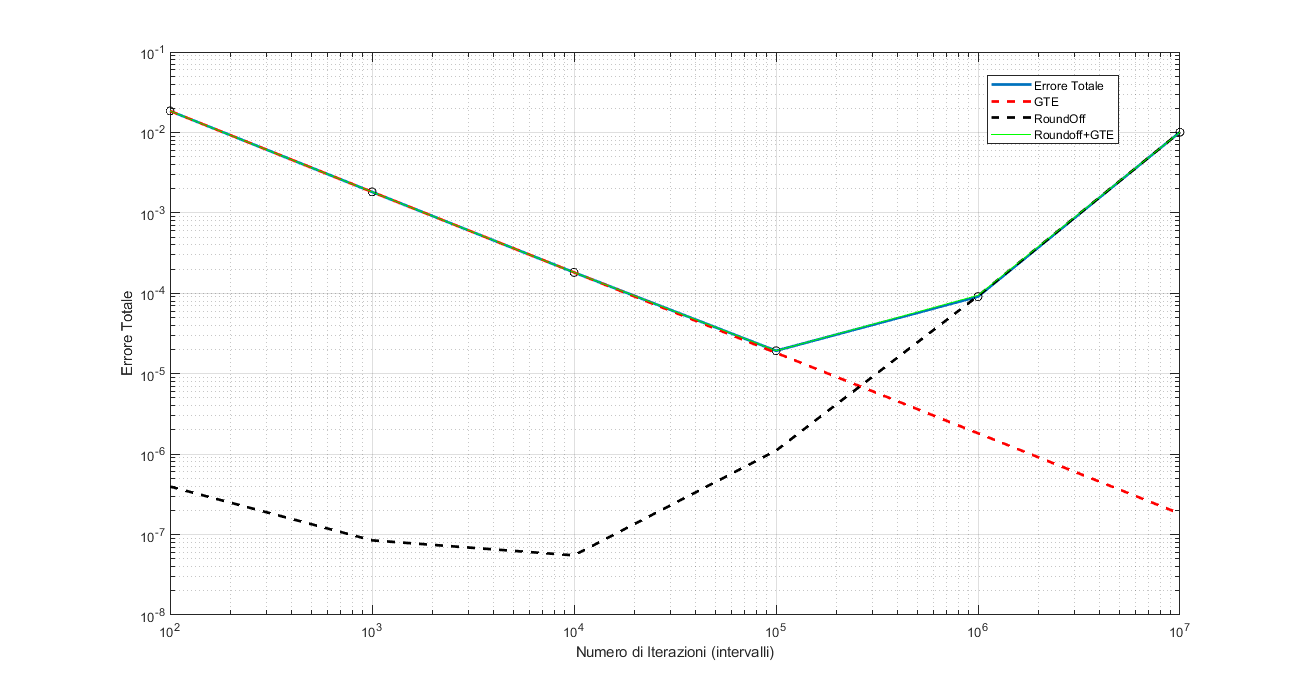
\includegraphics[width=\textwidth]{matlab/esercizio2_errori_confronto.png}
	\caption{\textit{Confronto degli errori}}
\end{figure}
Per $N=10^7$ si ha un errore di $10^{-2}$. 
\\In questo caso il valore di $N$ ottimo è:
\begin{equation*}
	10^5 < N_{opt} < 10^6
\end{equation*}

	
	
	\backmatter							%Fine numerazione capitoli (Per le conclusioni, Appendici ecc)
	

	
\end{document}